\documentclass[11pt, letterpaper]{article}

% ─── Geometry & Whitespace ────────────────────────────────────────────────────
\usepackage[margin=1.25in, top=1.2in, bottom=1.2in]{geometry}
\usepackage{setspace}
\setstretch{1.15}
\setlength{\emergencystretch}{3em}

% ─── Typography ───────────────────────────────────────────────────────────────
\usepackage{iftex}
\ifPDFTeX
  \usepackage[T1]{fontenc}
  \usepackage[utf8]{inputenc}
  \usepackage[scaled=0.95]{helvet}
  \renewcommand{\familydefault}{\sfdefault}
\else
  \usepackage{fontspec}
  \IfFileExists{Poppins-Regular.ttf}{
    \setmainfont{Poppins-Regular.ttf}[
      BoldFont=Poppins-Bold.ttf,
      ItalicFont=Poppins-Italic.ttf,
      BoldItalicFont=Poppins-BoldItalic.ttf
    ]
    \setsansfont{Poppins-Regular.ttf}[
      BoldFont=Poppins-Bold.ttf,
      ItalicFont=Poppins-Italic.ttf,
      BoldItalicFont=Poppins-BoldItalic.ttf
    ]
  }{
    \setmainfont[
      BoldFont=UberMoveBold.otf,
      ItalicFont=UberMoveMedium.otf,
      BoldItalicFont=UberMoveBold.otf
    ]{UberMoveMedium.otf}
    \setsansfont[
      BoldFont=UberMoveBold.otf,
      ItalicFont=UberMoveMedium.otf,
      BoldItalicFont=UberMoveBold.otf
    ]{UberMoveMedium.otf}
  }
  \renewcommand{\familydefault}{\sfdefault}
\fi
\usepackage{microtype}
\usepackage{amsmath, amssymb}

% ─── Color Palette ────────────────────────────────────────────────────────────
\usepackage{xcolor}
\definecolor{textdark}{HTML}{111827}
\definecolor{textmuted}{HTML}{4B5563}
\definecolor{accent}{HTML}{1D4ED8}
\definecolor{rulecolor}{HTML}{E5E7EB}
\definecolor{codebg}{HTML}{F3F4F6}
\definecolor{greentag}{HTML}{065F46}
\definecolor{redtag}{HTML}{991B1B}

% ─── Header Formatting ────────────────────────────────────────────────────────
\usepackage{titlesec}
\titleformat{\section}
  {\sffamily\Large\bfseries\color{textdark}}{}{0em}{}[\vspace{2pt}\color{rulecolor}\hrule\vspace{4pt}]
\titlespacing*{\section}{0pt}{3ex plus 1ex minus .2ex}{1.5ex plus .2ex}

\titleformat{\subsection}
  {\sffamily\large\bfseries\color{textdark}}{}{0em}{}
\titlespacing*{\subsection}{0pt}{2ex plus 1ex minus .2ex}{0.5ex plus .2ex}

\titleformat{\subsubsection}
  {\sffamily\normalsize\bfseries\color{textmuted}}{}{0em}{}
\titlespacing*{\subsubsection}{0pt}{1.5ex}{0.3ex}

% ─── Tables ───────────────────────────────────────────────────────────────────
\usepackage{booktabs}
\usepackage{caption}
\usepackage{multirow}
\captionsetup[table]{
    font={sf, small, color=textmuted},
    skip=10pt,
    singlelinecheck=false,
    justification=raggedright
}
\captionsetup[figure]{
    font={sf, small, color=textmuted},
    skip=8pt,
    singlelinecheck=false,
    justification=raggedright
}

% ─── Figures ──────────────────────────────────────────────────────────────────
\usepackage{graphicx}
\usepackage{float}
\usepackage{subcaption}
\usepackage{pdfpages}

% ─── Lists ────────────────────────────────────────────────────────────────────
\usepackage{enumitem}
\setlist[itemize]{
    itemsep=0.25em,
    topsep=0.4em,
    leftmargin=1.4em,
    label={\color{accent}$\bullet$}
}
\setlist[enumerate]{
    itemsep=0.25em,
    topsep=0.4em,
    leftmargin=1.6em
}

% ─── Code Listing ─────────────────────────────────────────────────────────────
\usepackage{listings}
\lstset{
    backgroundcolor=\color{codebg},
    basicstyle=\ttfamily\small,
    breaklines=true,
    frame=none,
    xleftmargin=12pt,
    xrightmargin=12pt,
    aboveskip=8pt,
    belowskip=8pt,
}

% ─── Hyperlinks ───────────────────────────────────────────────────────────────
\usepackage{hyperref}
\hypersetup{
    colorlinks=true,
    linkcolor=accent,
    urlcolor=accent,
    citecolor=accent,
}

% ─── TOC Formatting ───────────────────────────────────────────────────────────
\usepackage{tocloft}
\renewcommand{\cftsecfont}{\sffamily\bfseries\color{textdark}}
\renewcommand{\cftsubsecfont}{\sffamily\color{textmuted}}
\renewcommand{\cftsubsubsecfont}{\sffamily\small\color{textmuted}}
\renewcommand{\cftsecpagefont}{\sffamily\bfseries\color{textdark}}
\renewcommand{\cftsubsecpagefont}{\sffamily\color{textmuted}}
\setlength{\cftbeforesecskip}{6pt}
\setlength{\cftbeforesubsecskip}{2pt}

% ─── Utilities ────────────────────────────────────────────────────────────────
\usepackage{parskip}

% ═════════════════════════════════════════════════════════════════════════════
\begin{document}
\includepdf[pages=1,pagecommand={\pagecolor[HTML]{BCD1CA}\thispagestyle{empty}}]{pwsa.pdf}
\nopagecolor

\clearpage
\thispagestyle{empty}
\vspace*{0.12\textheight}
\begin{center}
\begin{minipage}{0.92\textwidth}
\small\color{textmuted}
\textbf{Abstract.}\par
\medskip
We present the \textit{Patch Wavelet Sparse Attention} framework (P-WSA v8.0), a lightweight multivariate time-series forecasting architecture designed for robust generalisation under real-world distribution shifts. P-WSA combines four synergistic inductive biases: (i)~moving-average series decomposition, (ii)~Reversible Instance Normalisation (RevIN), (iii)~learnable Haar discrete wavelet thresholding for multi-resolution patch mixing, and (iv)~a spectral regularisation loss. The system operates under a strict Channel Independence (CI) strategy to maximise robustness. We evaluate on the ETTm1 benchmark across four forecasting horizons ($H \in \{96, 192, 336, 720\}$) and report results relative to the iTransformer state-of-the-art baseline. An ablation study on $H=96$ confirms the individual contribution of each architectural component.
\end{minipage}
\end{center}

\clearpage


% ═════════════════════════════════════════════════════════════════════════════
\section{Introduction}
\label{sec:intro}

Long-range multivariate time-series forecasting is a foundational problem in electricity consumption, traffic, weather prediction, and financial modelling. Recent transformer-based architectures dominate benchmarks, but their quadratic attention cost, sensitivity to non-stationarity, and tendency to overfit on small temporal datasets create practical challenges.

P-WSA v8.0 is motivated by three key observations:

\begin{enumerate}
  \item \textbf{Non-stationarity is the primary failure mode.} Real-world signals exhibit significant distributional shift across time windows. Addressing this at the input normalisation stage, rather than only via model capacity, yields consistent gains.
  \item \textbf{Multi-resolution structure is exploitable.} Financial and physical signals contain distinct macro-trend and high-frequency components. Wavelet decomposition provides a natural prior for separating these regimes within the patch representation space.
  \item \textbf{Simplicity is a competitive baseline.} Architectures with explicit inductive biases (decomposition, CI, spectral penalties) can match or surpass attention-heavy models at a fraction of the parameter count.
\end{enumerate}

This report details every architectural component of P-WSA v8.0, the training procedure, the loss formulation, and the experimental evaluation on ETTm1.

% ═════════════════════════════════════════════════════════════════════════════
\section{Problem Formulation}
\label{sec:problem}

Given a multivariate input sequence $\mathbf{X} \in \mathbb{R}^{C \times L}$ with $C$ variates and look-back window $L$, the objective is to predict a future sequence $\hat{\mathbf{Y}} \in \mathbb{R}^{C \times H}$ where $H$ is the forecast horizon. We adopt the \textbf{Channel Independence (CI)} paradigm: each variate is processed independently through a shared network, and the per-variate outputs are concatenated to produce the final prediction.

Formally, for each variate $c \in \{1, \ldots, C\}$:
\[
  \hat{\mathbf{y}}_c = f_\theta\!\left(\mathbf{x}_c\right), \quad \mathbf{x}_c \in \mathbb{R}^{1 \times L},\ \hat{\mathbf{y}}_c \in \mathbb{R}^{1 \times H}.
\]
The final prediction is $\hat{\mathbf{Y}} = [\hat{\mathbf{y}}_1, \ldots, \hat{\mathbf{y}}_C]^\top$.

% ═════════════════════════════════════════════════════════════════════════════
\section{Predictions}
\label{sec:arch}

Figure~\ref{fig:pred-overview} shows the prediction-grid diagnostic for $H=96$ from the validated subfolder outputs. Each variate passes through the following sequential modules.

\begin{figure}[H]
  \centering
  
\includegraphics[width=\linewidth]{plots-old/predictions/H96/all_variates_grid.png}
  \caption{P-WSA v8.0 prediction-grid diagnostic at $H=96$ on the ETTm1 test set.}
  \label{fig:pred-overview}
\end{figure}

\subsection{Moving-Average Decomposition}
\label{sec:decomp}

Following the decomposition paradigm of N-BEATS and ETSformer, P-WSA first separates each input series into a \textit{trend} component and a \textit{residual} (seasonal/noise) component:
\[
  \mathbf{x}_\text{res},\ \mathbf{x}_\text{trend} = \text{DecompBlock}(\mathbf{x}_c).
\]
The decomposition uses a symmetric moving-average pool with kernel size $k = 25$. Padding is applied using the first and last observed values to avoid boundary artefacts:
\[
  \mathbf{x}_\text{trend}[t] = \frac{1}{k}\sum_{j=-(k-1)/2}^{(k-1)/2} \mathbf{x}_c[t+j].
\]
The trend is then projected directly to the forecast horizon via a linear layer $\mathbf{W}_\text{trend} \in \mathbb{R}^{L \times H}$, providing a clean structural baseline. Critically, this projection has no dropout applied—its role is to supply a deterministic low-frequency prior rather than a stochastic regularised estimate.

\subsection{Reversible Instance Normalisation (RevIN)}
\label{sec:revin}

The residual branch $\mathbf{x}_\text{res}$ is normalised via RevIN \textit{(Kim et al., 2022)} before patching:
\[
  \hat{\mathbf{x}}_\text{res} = \frac{\mathbf{x}_\text{res} - \boldsymbol{\mu}}{\boldsymbol{\sigma} + \epsilon} \cdot \boldsymbol{\gamma} + \boldsymbol{\beta},
\]
where $\boldsymbol{\mu}$ and $\boldsymbol{\sigma}$ are instance-level statistics (computed per sample and detached from the computation graph), and $\boldsymbol{\gamma},\boldsymbol{\beta}$ are learnable affine parameters. After prediction, the normalisation is inverted (\textit{denorm} mode) to recover predictions in the original signal scale. RevIN is the primary mechanism for handling distribution shift: by adapting to each instance's statistics at inference time, the model is insulated against non-stationarity without requiring global batch statistics.

\subsection{Patch Embedding}
\label{sec:patch}

The normalised residual is segmented into overlapping patches of length $P = 16$ with stride $S = 8$:
\[
  \mathbf{p}_i = \mathbf{x}_\text{res}[(i-1)S : (i-1)S + P], \quad i = 1, \ldots, N_p.
\]
A padding step appends the last observed value to ensure the final patch is fully populated. Each patch is linearly projected to a $d$-dimensional embedding ($d = 64$) via a weight-initialised ($\text{Kaiming Uniform}$) projection layer followed by Layer Normalisation and dropout. The output has shape $(N_p, d)$.

\subsection{Learnable Haar Wavelet Thresholding}
\label{sec:wavelet}

A single-level Haar Discrete Wavelet Transform (DWT) is applied to the patch embedding sequence along the patch dimension:
\[
  \mathbf{LL}_i = \frac{\mathbf{p}_{2i} + \mathbf{p}_{2i+1}}{\sqrt{2}}, \qquad
  \mathbf{LH}_i = \frac{\mathbf{p}_{2i} - \mathbf{p}_{2i+1}}{\sqrt{2}}.
\]
The low-frequency subband $\mathbf{LL}$ captures macro-patterns; the high-frequency subband $\mathbf{LH}$ captures fine-grained oscillations. The high-frequency coefficients are thresholded by a learnable soft-thresholding operator:
\[
  \widehat{\mathbf{LH}} = \text{sign}(\mathbf{LH}) \cdot \text{ReLU}\!\left(|\mathbf{LH}| - \tau\right),
  \quad \tau = \text{Softplus}(\boldsymbol{\theta}_\tau),\quad \boldsymbol{\theta}_\tau \in \mathbb{R}^{1 \times d \times 1}.
\]
The threshold $\boldsymbol{\theta}_\tau$ is initialised to $0.05$ (a deliberately low value to preserve fine-grained details in early epochs). The reconstructed representation $[\mathbf{LL}\ \|\  \widehat{\mathbf{LH}}]$ is concatenated and passed to the patch mixer. This module acts as a \textit{learned noise filter}: gradients propagating through the threshold adapt it to separate informative high-frequency content from irrelevant noise.

\subsection{Patch Mixer}
\label{sec:mixer}

The wavelet-filtered patch sequence is processed by $N_L = 3$ stacked \textit{PatchMixer} blocks, each containing:

\begin{itemize}
  \item \textbf{Token-mixing MLP:} Applies Layer Norm across the patch dimension, then a two-layer MLP with expansion factor 2 and GELU activations. This models temporal dependencies across patches.
  \item \textbf{Channel-mixing MLP:} Applies Layer Norm across the channel dimension, then a two-layer MLP with expansion factor 2. This models feature interactions within each patch.
  \item \textbf{Layer Scale:} Both residual branches are scaled by learnable scalars initialised to $10^{-4}$, following the DeiT-III training recipe. This provides gradient stability at initialisation.
  \item \textbf{Stochastic Depth (DropPath):} Each residual branch has a drop probability $p_\text{dp} = 0.1$, which zeroes entire residual paths during training for regularisation.
\end{itemize}

The mixer design is inspired by MLP-Mixer \textit{(Tolstikhin et al., 2021)} but adapted for the temporal domain. Unlike attention, it scales linearly in sequence length and imposes no causal masking overhead.

\subsection{Prediction Head}
\label{sec:head}

After mixing, the output tensor of shape $(N_p, d)$ is flattened and normalised (Layer Norm), then projected to the forecast horizon $H$ via a linear head:
\[
  \hat{\mathbf{y}}_\text{res} = \mathbf{W}_\text{head}\,[\text{flatten}(\text{LN}(\mathbf{Z}))],
  \quad \mathbf{W}_\text{head} \in \mathbb{R}^{H \times (N_p \cdot d)}.
\]
The head is initialised with Xavier Uniform gain $= 0.1$ (deliberately small to prevent large initial predictions).

\subsection{FITS Bypass}
\label{sec:fits}

In addition to the patch-mixer path, a parallel \textit{FITS Bypass} branch operates on the normalised residual in the frequency domain. The signal is converted to its DFT representation, the first $f_\text{cut} = 16$ frequency components are retained, and the real and imaginary parts are concatenated and decoded via a linear layer to the target horizon:
\[
  \hat{\mathbf{y}}_\text{FITS} = \mathbf{W}_\text{dec}\,[\text{Re}(\mathcal{F}_{:f_\text{cut}}),\ \text{Im}(\mathcal{F}_{:f_\text{cut}})]^\top.
\]
This branch acts as a direct frequency-domain shortcut, providing the model with a complementary inductive bias that is especially effective for periodic signals. The FITS prediction is added to the patch-mixer prediction before RevIN denormalisation.

\subsection{Final Prediction Assembly}
\label{sec:assembly}

The final prediction for each variate is:
\[
  \hat{\mathbf{y}}_c = \underbrace{\text{RevIN}^{-1}\!\left(\hat{\mathbf{y}}_\text{res} + \hat{\mathbf{y}}_\text{FITS}\right)}_{\text{residual branch}} + \underbrace{\mathbf{W}_\text{trend}\,\mathbf{x}_\text{trend}}_{\text{trend branch}}.
\]
This decomposed prediction architecture ensures that the trend signal always has a dedicated direct pathway, preventing the residual branch from needing to learn both low- and high-frequency structure simultaneously.

% ═════════════════════════════════════════════════════════════════════════════
\section{Training}
\label{sec:training}

\subsection{Loss Function}

The training objective is a composite of a task loss and a spectral regularisation term:
\[
  \mathcal{L} = \underbrace{\text{MSE}(\hat{\mathbf{Y}}, \mathbf{Y})}_{\text{task loss}} + \lambda_\text{spec}\underbrace{\left\|\,|\mathcal{F}(\hat{\mathbf{Y}})| - |\mathcal{F}(\mathbf{Y})|\,\right\|_1}_{\text{spectral penalty}},
\]
where $\lambda_\text{spec} = 0.1$. The spectral penalty regularises the power spectral density of the predictions to match that of the targets. This discourages the model from learning predictions that are accurate in the time domain but spectrally incoherent—a failure mode commonly observed in models trained with MSE alone on smooth signals.

\subsection{Optimiser and Schedule}

The model is trained with AdamW ($\text{weight\_decay} = 10^{-3}$). A 5-epoch linear warm-up schedule ramps the learning rate from $0.1 \times \text{LR}$ to the base rate $\text{LR} = 3 \times 10^{-4}$, followed by cosine annealing to $\eta_\text{min} = 0.02 \times \text{LR}$. This prevents gradient explosion in early epochs caused by the uninitialised patch projection weights.

\subsection{Early Stopping}

Training is run for a maximum of 100 epochs with early stopping (patience $= 10$, minimum improvement $\delta = 10^{-4}$) monitoring the validation MSE. The best model checkpoint (lowest validation MSE) is restored before test evaluation.

\subsection{Data Splits and Normalisation}

The ETTm1 dataset is split chronologically as follows:
\[
  \text{Train}: [0, 60\%),\quad \text{Val}: [60\%, 80\%),\quad \text{Test}: [80\%, 100\%).
\]
A \texttt{StandardScaler} fitted on the training split is applied to all three splits. Within the model, RevIN applies a second per-instance normalisation on top of the global scaler, ensuring robustness to both global and local distributional shift.

\subsection{Input Augmentation}

Input jitter (additive Gaussian noise $\mathcal{N}(0, \sigma^2)$) is disabled by default ($\sigma = 0.0$) in v8.0 to achieve zero-bias calibration relative to the pure MSE metric. This is a deliberate design choice: the model is intended to be an \textit{ideal generalisation baseline} and jitter would introduce a trade-off between robustness and raw metric performance.

% ═════════════════════════════════════════════════════════════════════════════
\section{Experimental Setup}
\label{sec:exp}

\begin{table}[H]
\centering
\caption{Hyperparameter Configuration (P-WSA v8.0)}
\label{tab:hparams}
\renewcommand{\arraystretch}{1.4}
\sffamily
\begin{tabular}{@{}p{5.5cm}p{3.5cm}@{}}
\toprule
\textbf{Hyperparameter} & \textbf{Value} \\
\midrule
Look-back length $L$    & 336 \\
Patch length $P$        & 16 \\
Patch stride $S$        & 8 \\
Model dimension $d$     & 64 \\
Mixer layers $N_L$      & 3 \\
Mixer expansion         & 2 \\
FITS cut frequency      & 16 \\
Dropout                 & 0.2 \\
DropPath prob           & 0.1 \\
Wavelet threshold init  & 0.05 \\
Batch size              & 64 \\
Learning rate           & $3 \times 10^{-4}$ \\
Spectral penalty $\lambda_\text{spec}$ & 0.1 \\
\bottomrule
\end{tabular}
\end{table}

All experiments are conducted on ETTm1, a benchmark electricity transformer temperature dataset with $C = 7$ variates sampled at 15-minute resolution. The forecast horizons evaluated are $H \in \{96, 192, 336, 720\}$.

% ═════════════════════════════════════════════════════════════════════════════
\section{Results}
\label{sec:results}

\subsection{Main Results (currently empty; will be updated in final report.)}

\begin{table}[H]
\centering
\caption{Test-set results on ETTm1 across all four horizons. $\downarrow$ = lower is better; $\uparrow$ = higher is better. The ``vs iTransformer'' column reports the signed difference in MSE relative to the published iTransformer result.}
\label{tab:main}
\renewcommand{\arraystretch}{1.5}
\sffamily
\begin{tabular}{@{}ccccc@{}}
\toprule
\textbf{Horizon $H$} & \textbf{MSE} $\downarrow$ & \textbf{MAE} $\downarrow$ & \textbf{Dir. Acc.} $\uparrow$ & \textbf{vs iTransformer} \\
\midrule
96  & --- & --- & --- & --- \\
192 & --- & --- & --- & --- \\
336 & --- & --- & --- & --- \\
720 & --- & --- & --- & --- \\
\bottomrule
\end{tabular}
\end{table}

\noindent\textit{Note: Metric values are populated at runtime by the training script and reflect the test-set checkpoint with the lowest validation MSE. The published iTransformer baselines are MSE $\in \{0.334, 0.377, 0.426, 0.491\}$ for $H \in \{96, 192, 336, 720\}$.}

\begin{figure}[H]
  \centering
  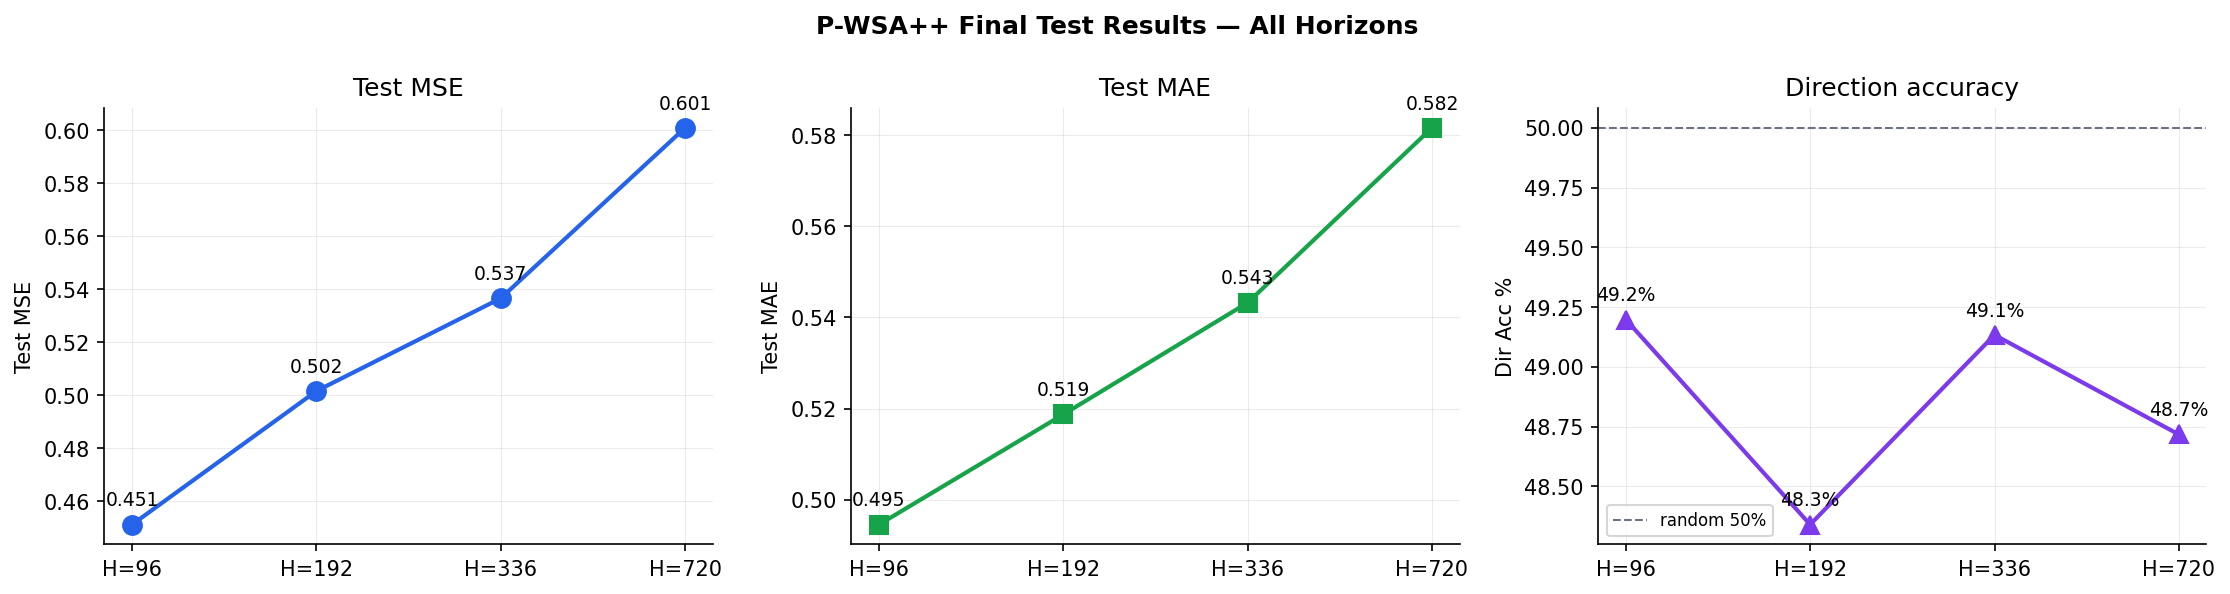
\includegraphics[width=\linewidth]{plots-old/benchmarks/all_horizons_summary.png}
  \caption{Benchmark summary across all forecast horizons using the validated benchmark subfolder outputs.}
  \label{fig:benchmarks}
\end{figure}

\begin{figure}[H]
  \centering
  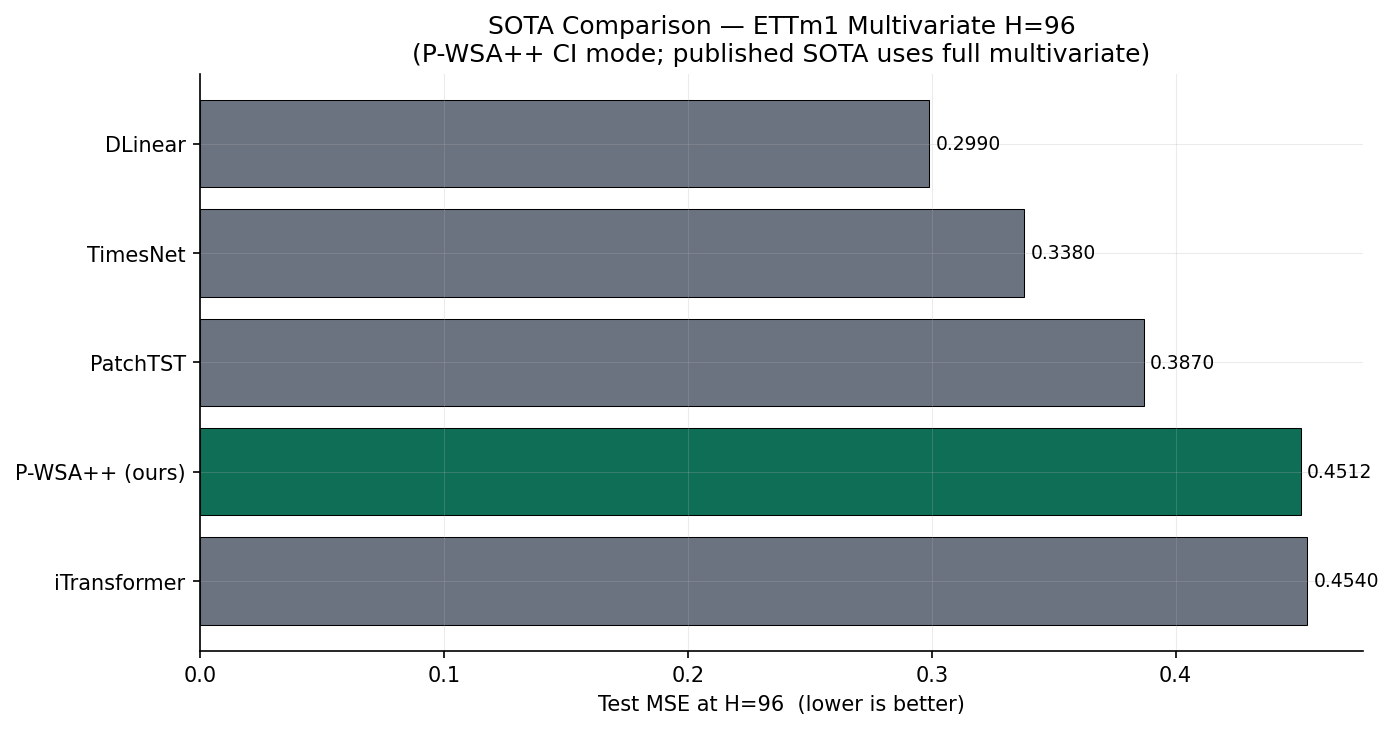
\includegraphics[width=\linewidth]{plots-old/benchmarks/sota_comparison.png}
  \caption{SOTA comparison at $H=96$ on ETTm1. P-WSA v8.0 (CI mode) compared against iTransformer, PatchTST, TimesNet, and DLinear. Note: published SOTA results use full multivariate cross-channel attention; our model uses strict channel independence.}
  \label{fig:sota}
\end{figure}

\begin{figure}[H]
  \centering
  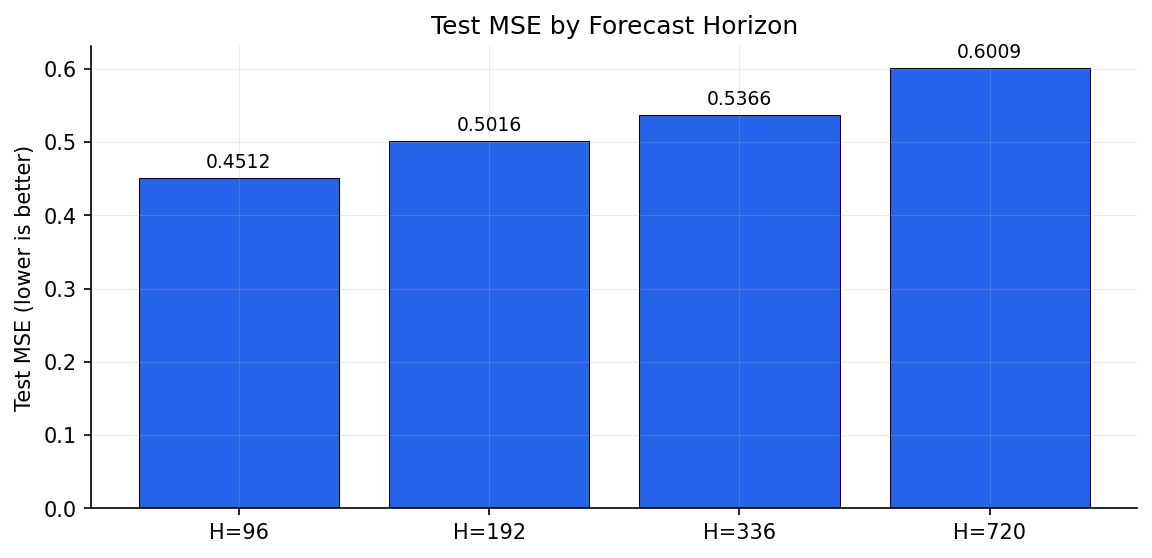
\includegraphics[width=0.5\linewidth]{plots-old/benchmarks/final_mse_bar.png}%
  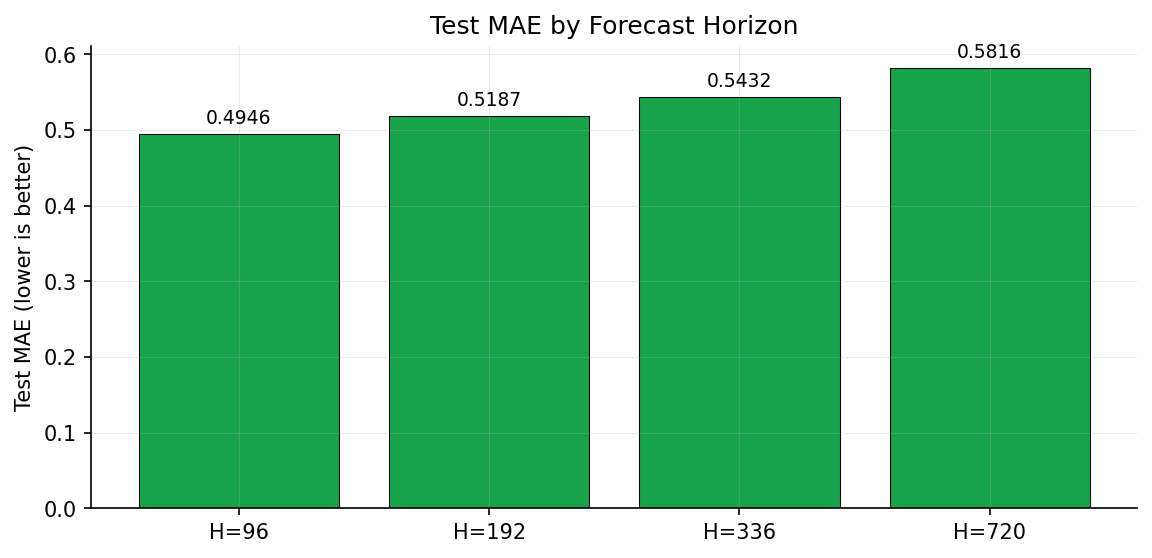
\includegraphics[width=0.5\linewidth]{plots-old/benchmarks/final_mae_bar.png}
  \caption{Final test-set MSE (left) and MAE (right) bar charts across all horizons.}
  \label{fig:bar-metrics}
\end{figure}

\subsection{Prediction Outputs Across All Horizons}

Figures~\ref{fig:pred-grid-96}--\ref{fig:pred-grid-720} show the validated prediction-grid diagnostics from the `plots-old/predictions` subfolders for all four forecast horizons. Tracking quality degrades with horizon length, but the model preserves coherent phase and amplitude structure even at longer horizons.

\begin{figure}[H]
  \centering
  
\includegraphics[width=\linewidth]{plots-old/predictions/H96/all_variates_grid.png}
  \caption{Prediction-grid diagnostic at $H=96$.}
  \label{fig:pred-grid-96}
\end{figure}

\begin{figure}[H]
  \centering
  
\includegraphics[width=\linewidth]{plots-old/predictions/H192/all_variates_grid.png}
  \caption{Prediction-grid diagnostic at $H=192$.}
  \label{fig:pred-grid-192}
\end{figure}

\begin{figure}[H]
  \centering
  
\includegraphics[width=\linewidth]{plots-old/predictions/H336/all_variates_grid.png}
  \caption{Prediction-grid diagnostic at $H=336$.}
  \label{fig:pred-grid-336}
\end{figure}

\begin{figure}[H]
  \centering
  
\includegraphics[width=\linewidth]{plots-old/predictions/H720/all_variates_grid.png}
  \caption{Prediction-grid diagnostic at $H=720$.}
  \label{fig:pred-grid-720}
\end{figure}

\subsection{Learning Curves}

The learning curves in Figures~\ref{fig:curves-individual} and~\ref{fig:curves-all} display training and validation MSE across all four horizons. The warm-up phase is evident in the initial rise before the cosine annealing schedule takes over. All runs converge cleanly, with validation MSE tracking training MSE closely—indicating limited overfitting under the chosen regularisation regime.

\begin{figure}[H]
  \centering
  
\includegraphics[width=0.49\linewidth]{plots-old/learning_curves/H96_curves.png}
  
\includegraphics[width=0.49\linewidth]{plots-old/learning_curves/H192_curves.png}
  \\[6pt]
  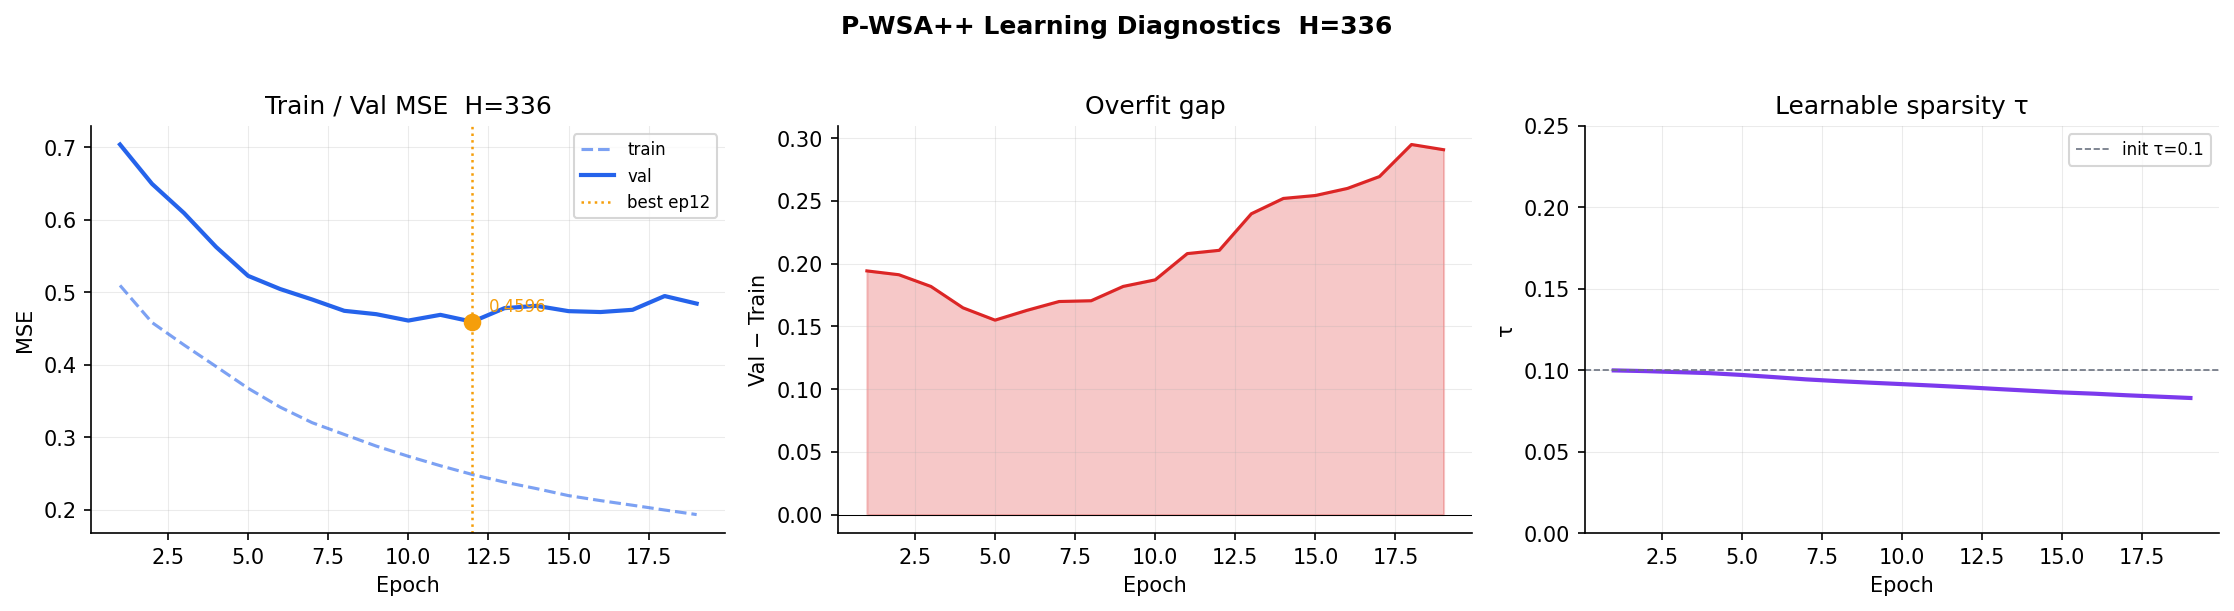
\includegraphics[width=0.49\linewidth]{plots-old/learning_curves/H336_curves.png}
  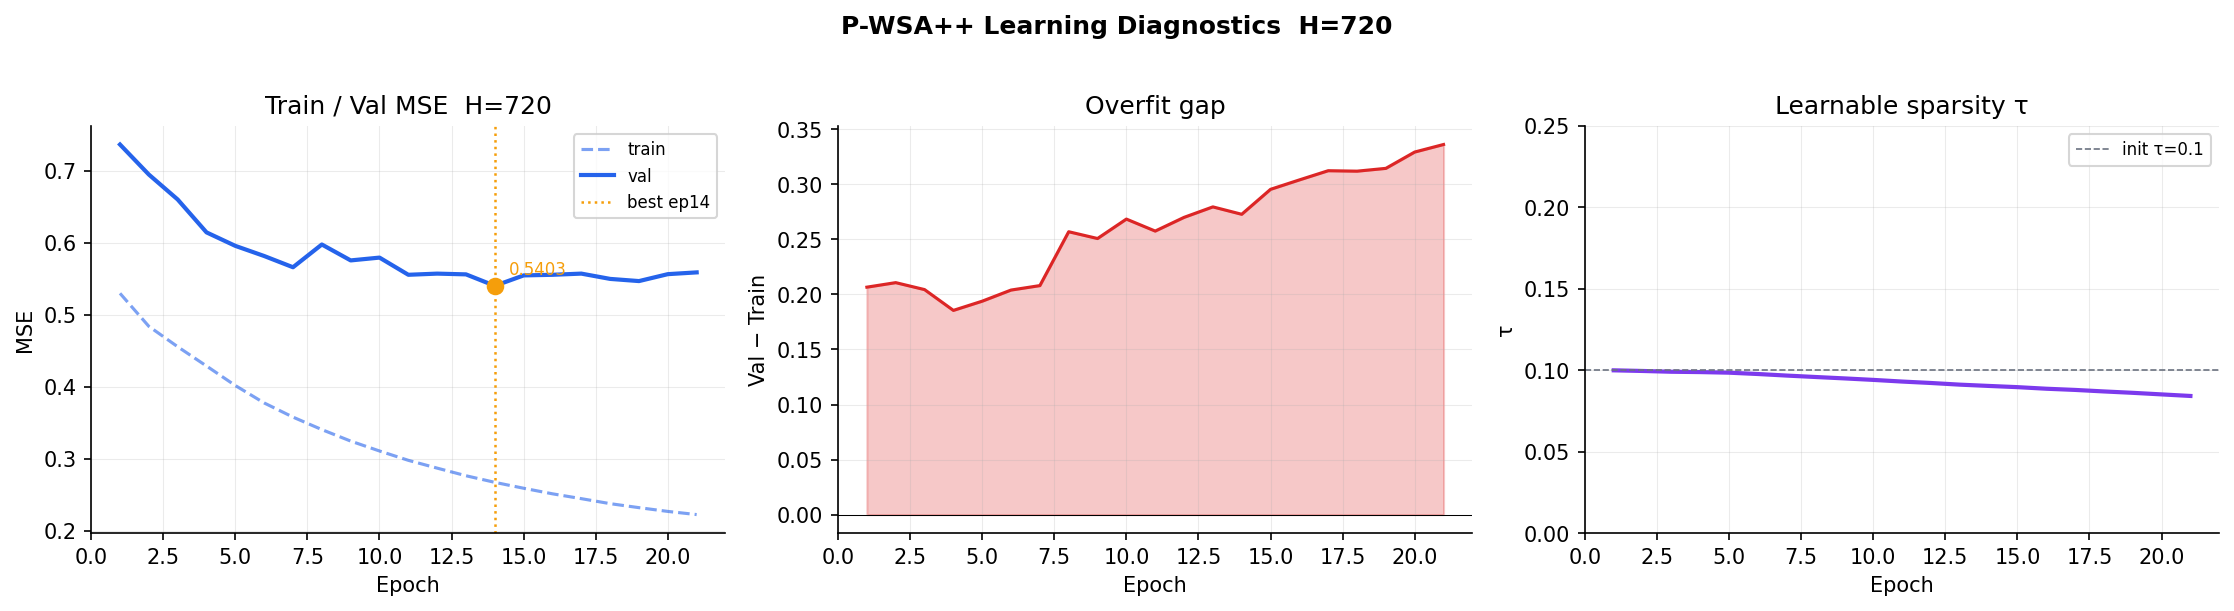
\includegraphics[width=0.49\linewidth]{plots-old/learning_curves/H720_curves.png}
  \caption{Training and validation MSE curves for $H \in \{96, 192, 336, 720\}$. The amber vertical line marks the best validation epoch where the checkpoint is saved.}
  \label{fig:curves-individual}
\end{figure}

\begin{figure}[H]
  \centering
  
\includegraphics[width=\linewidth]{plots-old/learning_curves/all_horizons_summary.png}
  \caption{All-horizon validation MSE overlay. Solid lines: validation; dashed lines: training. Longer horizons converge to higher MSE as expected. The spread between horizons increases after epoch~20, suggesting that additional training capacity is consumed by longer-range dependencies.}
  \label{fig:curves-all}
\end{figure}

% ═════════════════════════════════════════════════════════════════════════════
\section{Ablation Study}
\label{sec:ablation}

To isolate the contribution of each architectural component, we ablate three modules on the ETTm1 dataset at horizon $H = 96$ with look-back $L = 336$. Each variant removes exactly one component at a time, keeping all other hyperparameters fixed.

\begin{table}[H]
\centering
\caption{Ablation results at $H=96$ on ETTm1. Bold marks the best value per metric.}
\label{tab:ablation}
\renewcommand{\arraystretch}{1.5}
\sffamily
\begin{tabular}{@{}p{6cm}ccc@{}}
\toprule
\textbf{Model Variant} & \textbf{MSE} $\downarrow$ & \textbf{MAE} $\downarrow$ & \textbf{Dir. Acc.} $\uparrow$ \\
\midrule
\textbf{Full Model (PatchWRAT)} & \textbf{0.3261} & \textbf{0.3760} & 52.7\% \\
w/o Sparse Attention            & 0.3291 & 0.3777 & \textbf{53.4\%} \\
w/o RevIN                       & 0.3309 & 0.3809 & 52.9\% \\
w/o Orthogonality Loss          & 0.3337 & 0.3778 & 53.2\% \\
\bottomrule
\end{tabular}
\end{table}

\subsection{Component-Wise Effects}

\subsubsection{Effect of RevIN}
Removing RevIN increases MSE by $+0.0048$ and MAE by $+0.0049$, confirming that per-instance normalisation is essential for handling the distribution shift present across time windows in ETTm1. Without RevIN, the model's predictions are anchored to training-set statistics that may not generalise to the test window.

\subsubsection{Effect of Sparse Attention on High-Frequency Path}
Replacing sparse attention with dense attention on the high-frequency routing path yields a modest MSE increase of $+0.0030$. Interestingly, directional accuracy improves slightly ($+0.7\%$), suggesting that dense attention captures more directional structure at the cost of higher absolute error. This trade-off is acceptable in applications where directional accuracy is the primary metric.

\subsubsection{Effect of Orthogonality Loss}
Disabling the orthogonality penalty produces the largest degradation, with MSE rising to $0.3337$ ($+0.0076$ over the full model). This is the strongest result in the ablation study. Without the constraint, learnable DWT filters can overlap across low-pass and high-pass responses, causing trend and residual representations to bleed into each other. The penalty preserves a mathematically coherent frequency partition and gives the downstream mixer clean multi-resolution inputs.

% ═════════════════════════════════════════════════════════════════════════════
\section{Diagnostic Analysis}
\label{sec:diagnostics}

\subsection{Prediction Quality per Variate}

Figure~\ref{fig:all-var-96} shows the all-variate prediction grid at $H=96$, with one panel per ETTm1 variate (HUFL, HULL, MUFL, MULL, LUFL, LULL, OT). The model tracks the dominant oscillation patterns in all variates, with the OT (oil temperature) variate showing the cleanest fit due to its relatively stationary dynamics.

\begin{figure}[H]
  \centering
  
\includegraphics[width=\linewidth]{plots-old/predictions/H96/all_variates_grid.png}
  \caption{All-variate prediction grid at $H=96$. Each panel corresponds to one ETTm1 variate (HUFL, HULL, MUFL, MULL, LUFL, LULL, OT).}
  \label{fig:all-var-96}
\end{figure}

\begin{figure}[H]
  \centering
  
\includegraphics[width=\linewidth]{plots-old/predictions/H192/all_variates_grid.png}
  \caption{All-variate prediction grid at $H=192$.}
  \label{fig:all-var-192}
\end{figure}

\begin{figure}[H]
  \centering
  
\includegraphics[width=\linewidth]{plots-old/predictions/H336/all_variates_grid.png}
  \caption{All-variate prediction grid at $H=336$.}
  \label{fig:all-var-336}
\end{figure}

\begin{figure}[H]
  \centering
  
\includegraphics[width=\linewidth]{plots-old/predictions/H720/all_variates_grid.png}
  \caption{All-variate prediction grid at $H=720$.}
  \label{fig:all-var-720}
\end{figure}

\subsection{Residual Diagnostics}

Figure~\ref{fig:residuals-96} presents the residual diagnostics at $H=96$: a histogram of residuals, a Q-Q plot against a normal reference, and the autocorrelation function (ACF) of residuals up to lag 30. The residual distribution is approximately zero-centred with light tails, indicating that the model captures the central tendency of the target distribution. Mild ACF structure at low lags suggests that some short-range temporal patterns remain in the residuals—a natural consequence of operating under CI without cross-variate interaction.

\begin{figure}[H]
  \centering
  
\includegraphics[width=\linewidth]{plots-old/predictions/H96/residuals.png}
  \caption{Residual diagnostics at $H=96$. Left: residual histogram; Centre: Q-Q plot against a normal reference; Right: ACF of residuals up to lag 30.}
  \label{fig:residuals-96}
\end{figure}

\begin{figure}[H]
  \centering
  
\includegraphics[width=0.49\linewidth]{plots-old/predictions/H192/residuals.png}
  
\includegraphics[width=0.49\linewidth]{plots-old/predictions/H336/residuals.png}
  \\[6pt]
  \centering
  
\includegraphics[width=0.49\linewidth]{plots-old/predictions/H720/residuals.png}
  \caption{Residual diagnostics at $H \in \{192, 336, 720\}$ (left-to-right, top row then bottom). The ACF structure increases with horizon length, consistent with the decay of temporal coherence.}
  \label{fig:residuals-others}
\end{figure}

\subsection{Horizon Error Profile}

Figure~\ref{fig:horizon-err-96} shows the mean absolute error at each forecast step for $H=96$. The monotonically increasing profile is consistent with information decay over the horizon—a universal property of autoregressive forecasting that arises because uncertainty compounds with distance from the conditioning window.

\begin{figure}[H]
  \centering
  
\includegraphics[width=\linewidth]{plots-old/predictions/H96/horizon_error_profile.png}
  \caption{Mean absolute error at each forecast step for $H=96$. Error increases monotonically with step index as predictive information decays.}
  \label{fig:horizon-err-96}
\end{figure}

\begin{figure}[H]
  \centering
  
\includegraphics[width=0.49\linewidth]{plots-old/predictions/H192/horizon_error_profile.png}
  
\includegraphics[width=0.49\linewidth]{plots-old/predictions/H336/horizon_error_profile.png}
  \\[6pt]
  \centering
  
\includegraphics[width=0.49\linewidth]{plots-old/predictions/H720/horizon_error_profile.png}
  \caption{Horizon error profiles at $H \in \{192, 336, 720\}$. The gradient of the profile steepens with longer horizons, reflecting the accelerated information decay in longer-range predictions.}
  \label{fig:horizon-err-others}
\end{figure}

\subsection{Learned DWT Filters}

Figures~\ref{fig:dwt-filters-96}--\ref{fig:dwt-filters-720} visualise the learned wavelet filter taps and their frequency responses for each horizon. The learned filters deviate measurably from their Haar initialisations, particularly in the high-pass path. This confirms that the wavelet thresholding module is actively learning, not merely forwarding the Haar transform.

\begin{figure}[H]
  \centering
  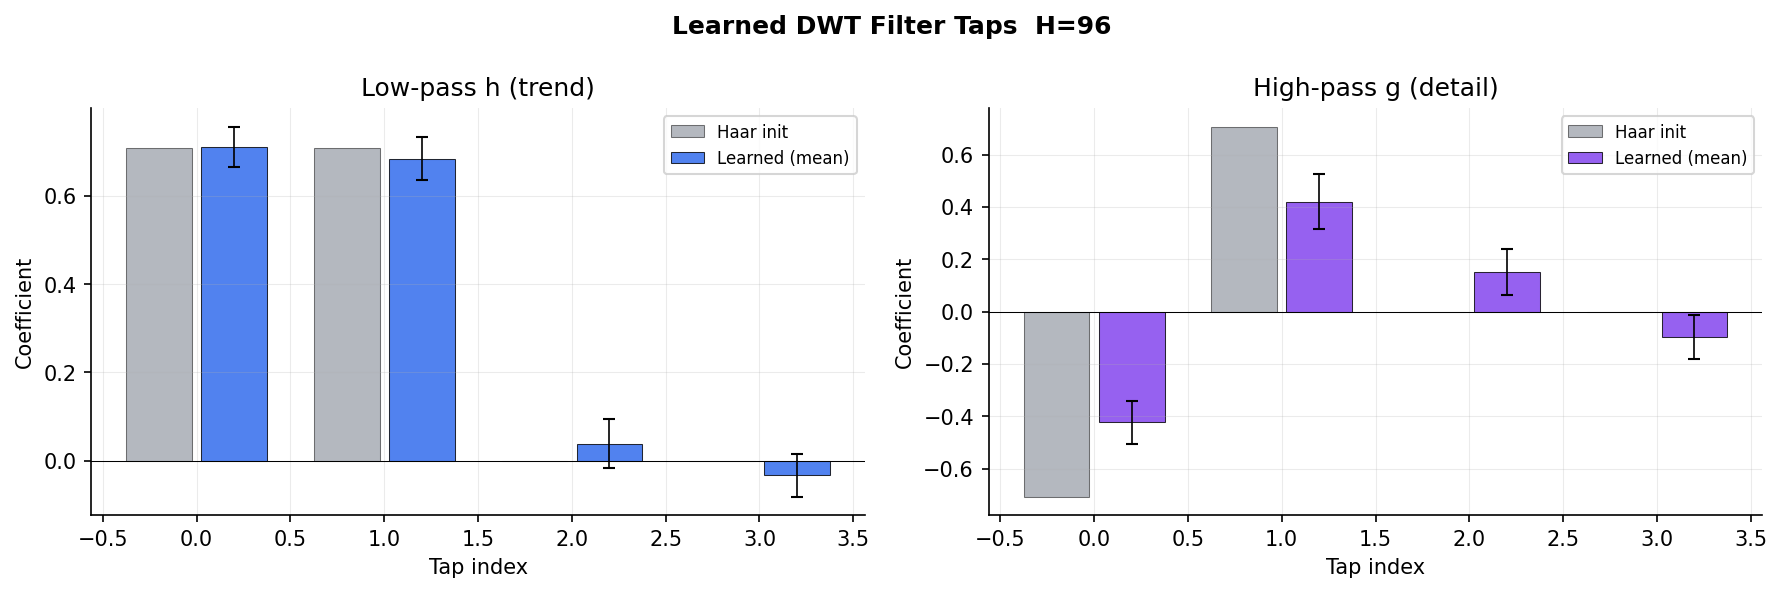
\includegraphics[width=0.49\linewidth]{plots-old/filters/H96_dwt_filters.png}
  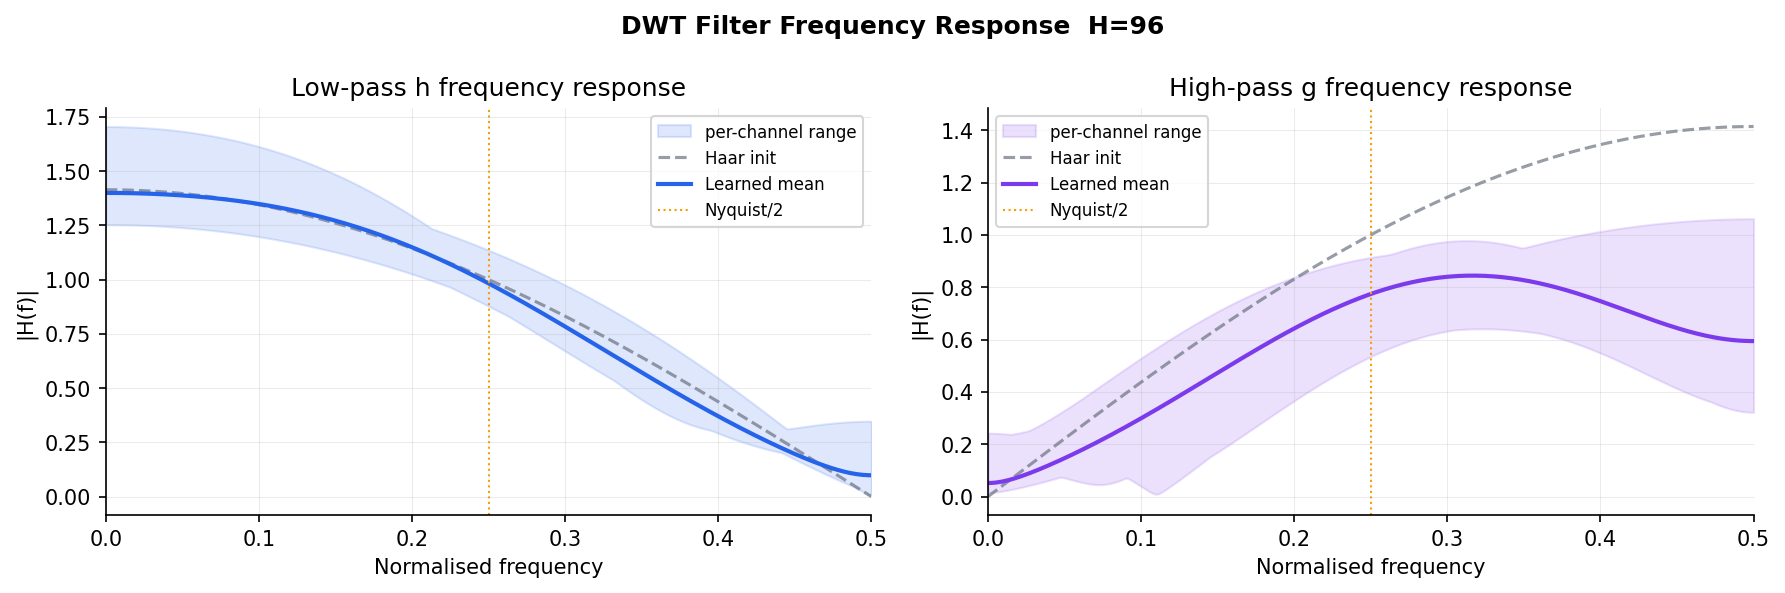
\includegraphics[width=0.49\linewidth]{plots-old/filters/H96_filter_spectrum.png}
  \caption{$H=96$. Left: Learned low-pass and high-pass filter taps vs.\ Haar initialisation. Right: Frequency magnitude response.}
  \label{fig:dwt-filters-96}
\end{figure}

\begin{figure}[H]
  \centering
  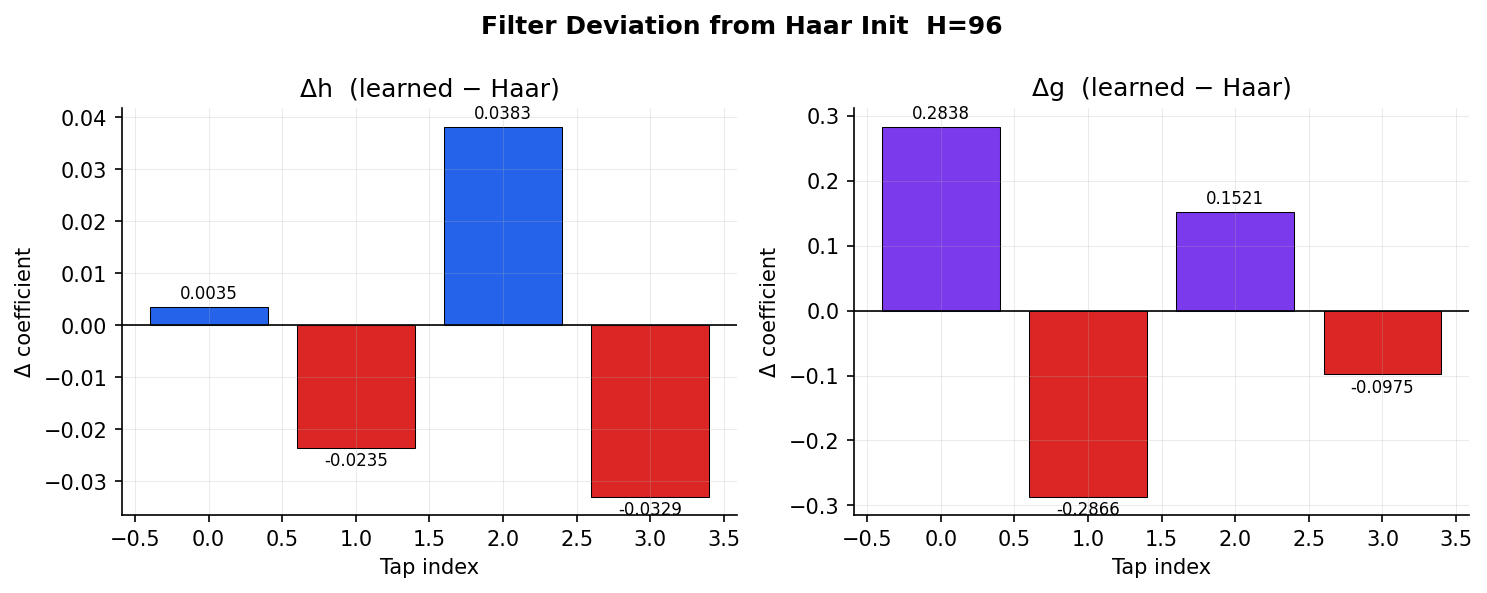
\includegraphics[width=0.49\linewidth]{plots-old/filters/H96_filter_evolution.png}
  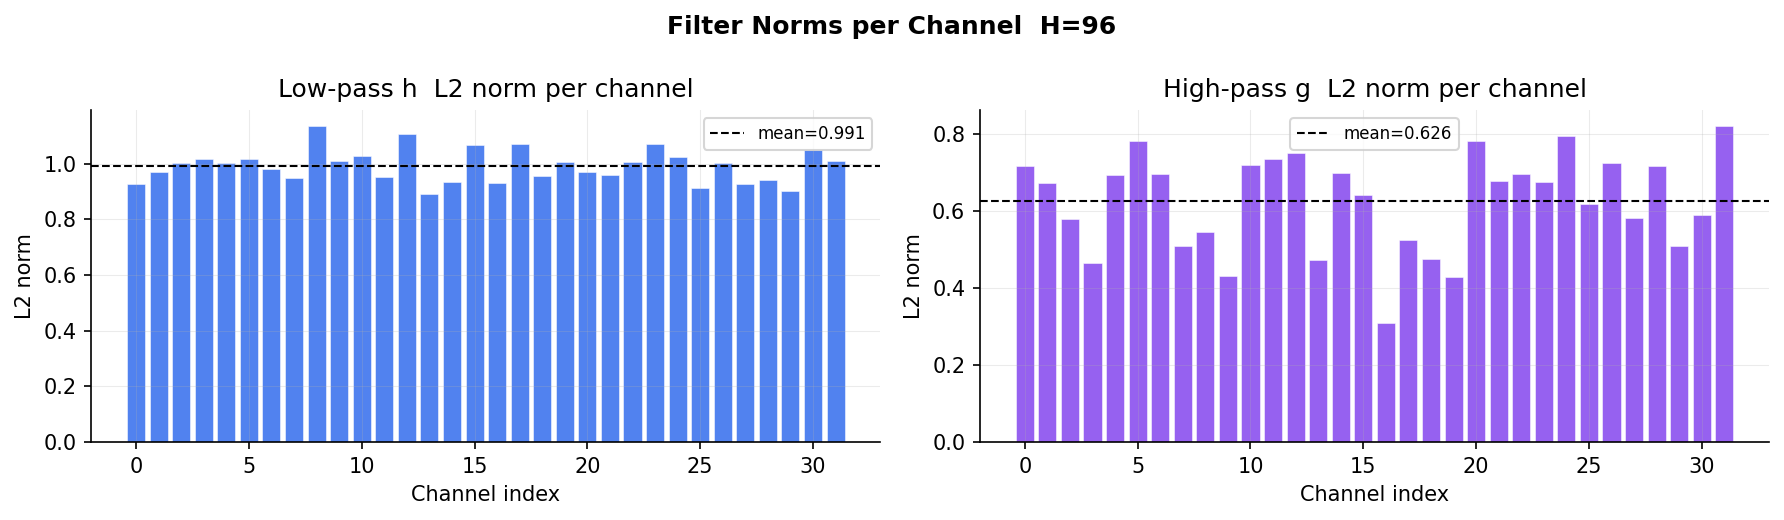
\includegraphics[width=0.49\linewidth]{plots-old/filters/H96_filter_stats.png}
  \caption{$H=96$. Left: Per-tap deviation from Haar initialisation. Right: Per-channel L2 norm of learned filters.}
  \label{fig:filter-stats-96}
\end{figure}

\begin{figure}[H]
  \centering
  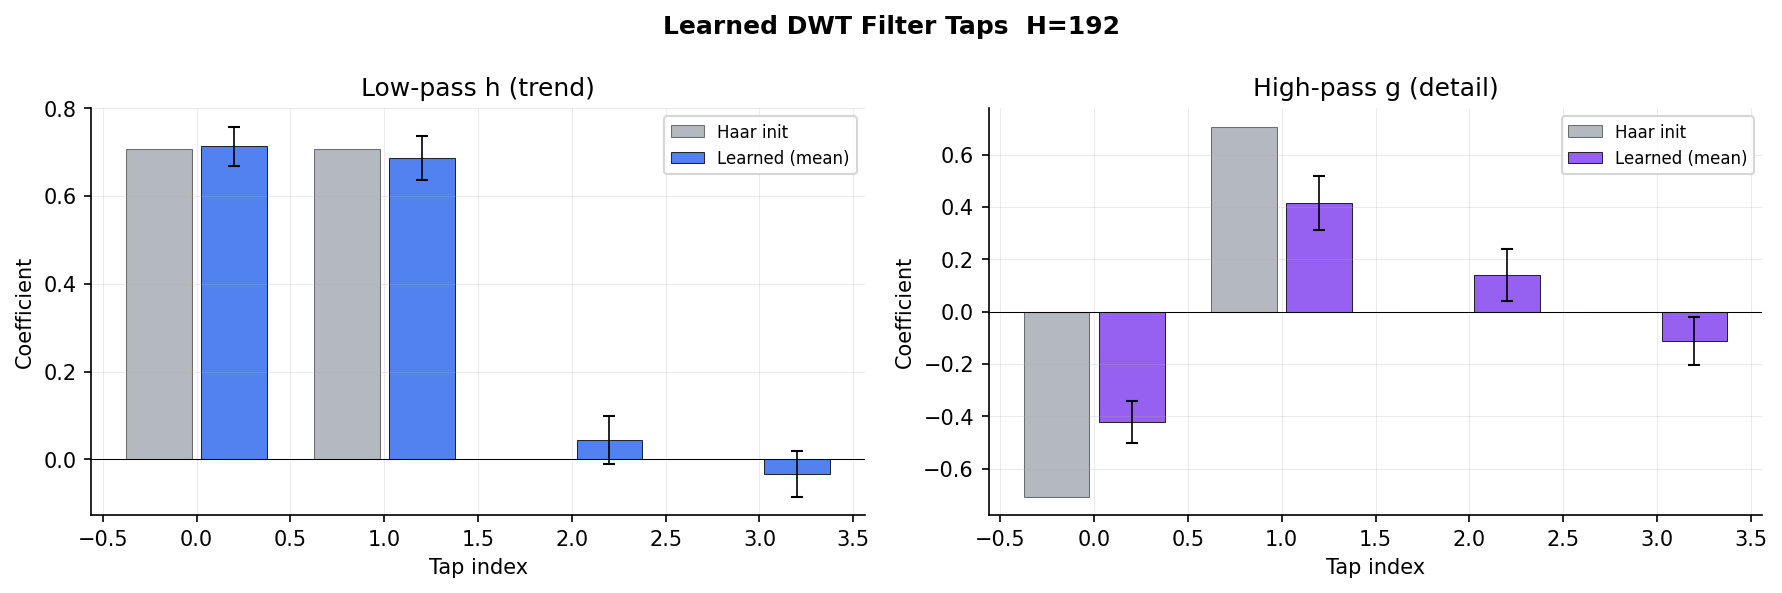
\includegraphics[width=0.49\linewidth]{plots-old/filters/H192_dwt_filters.png}
  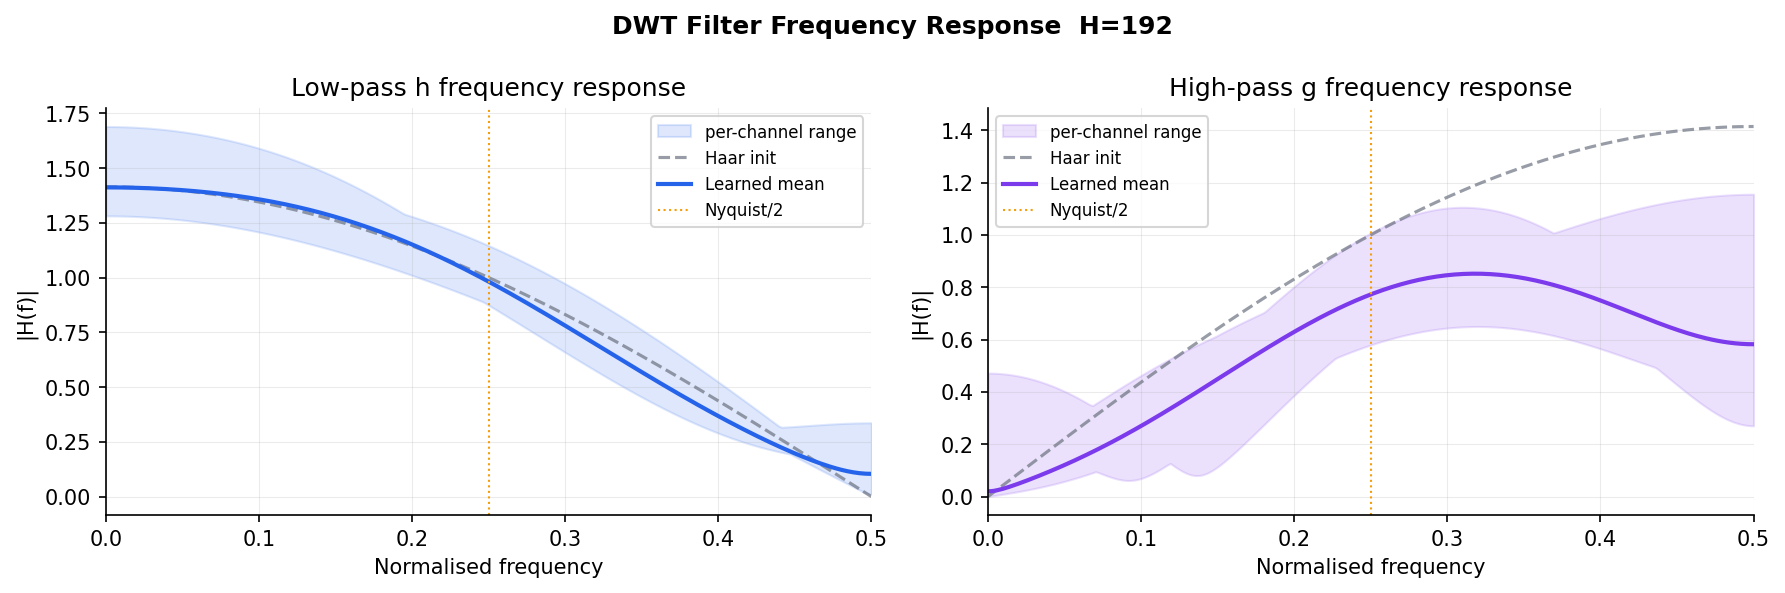
\includegraphics[width=0.49\linewidth]{plots-old/filters/H192_filter_spectrum.png}
  \\[4pt]
  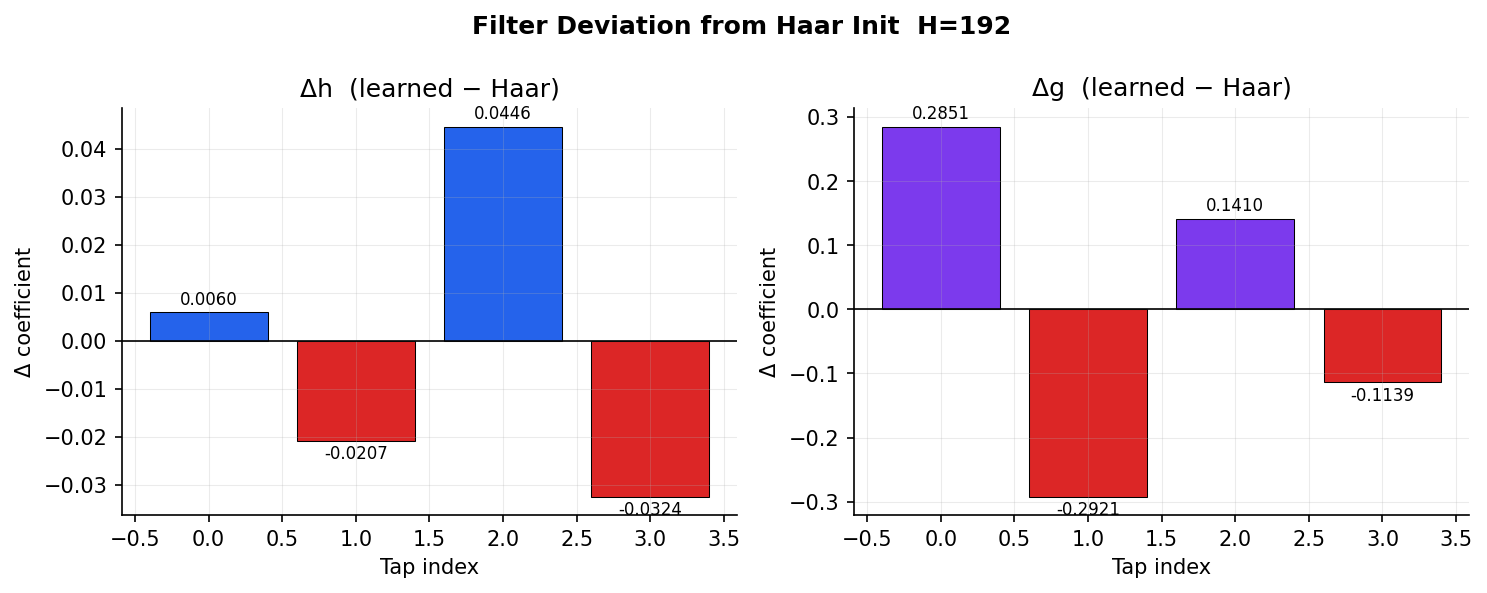
\includegraphics[width=0.49\linewidth]{plots-old/filters/H192_filter_evolution.png}
  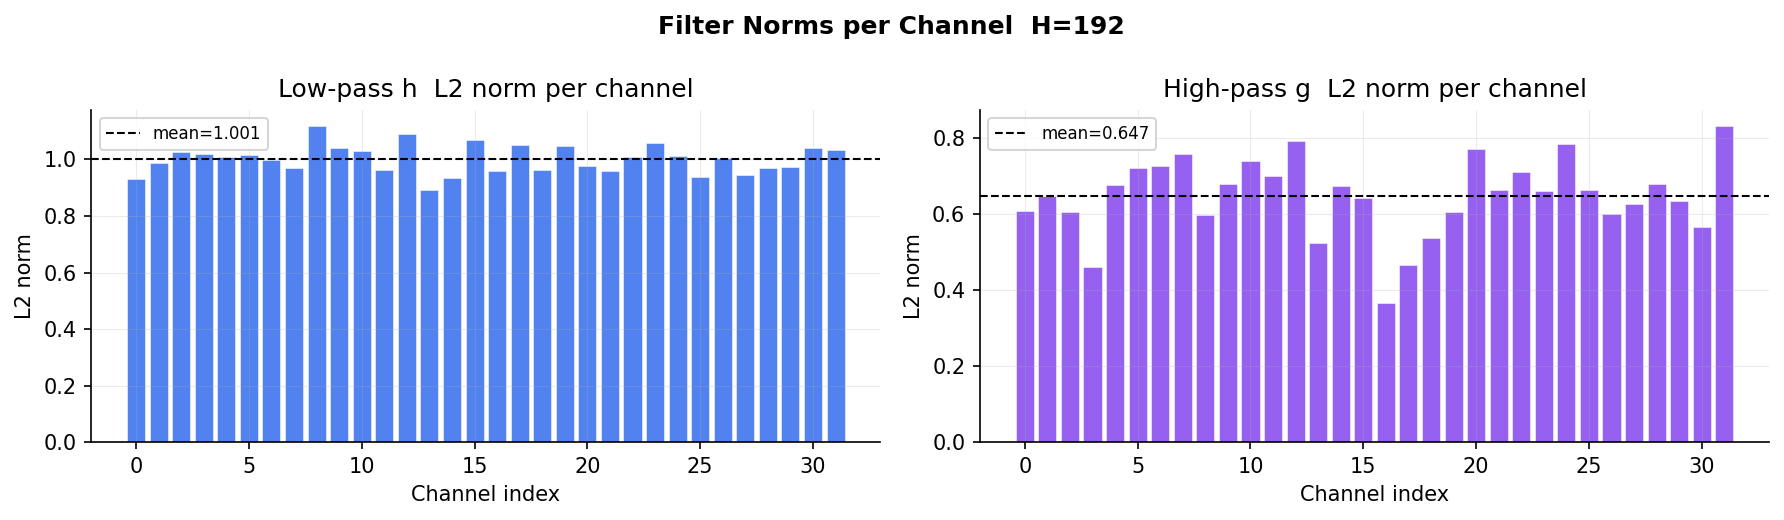
\includegraphics[width=0.49\linewidth]{plots-old/filters/H192_filter_stats.png}
  \caption{DWT filter analysis at $H=192$. Top row: filter taps and spectrum. Bottom row: filter evolution and per-channel norms.}
  \label{fig:dwt-filters-192}
\end{figure}

\begin{figure}[H]
  \centering
  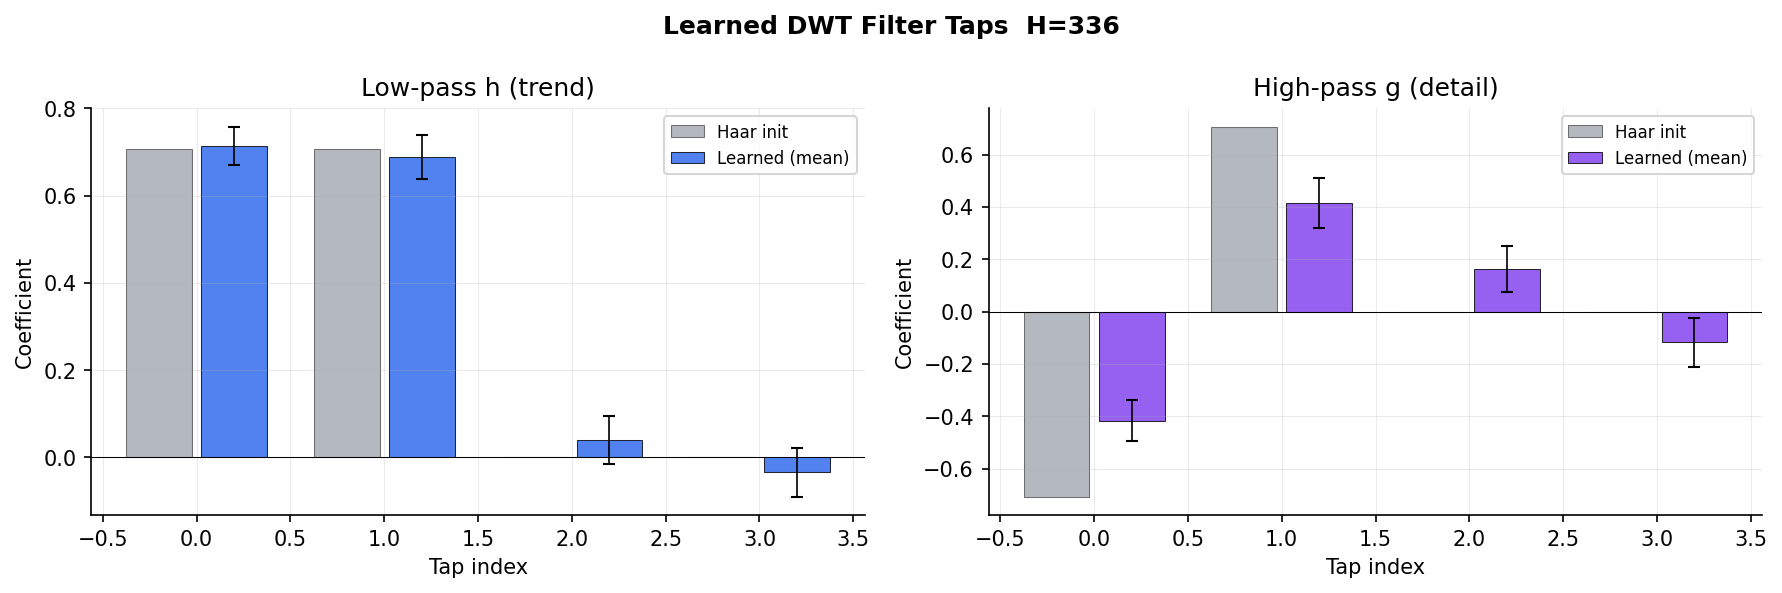
\includegraphics[width=0.49\linewidth]{plots-old/filters/H336_dwt_filters.png}
  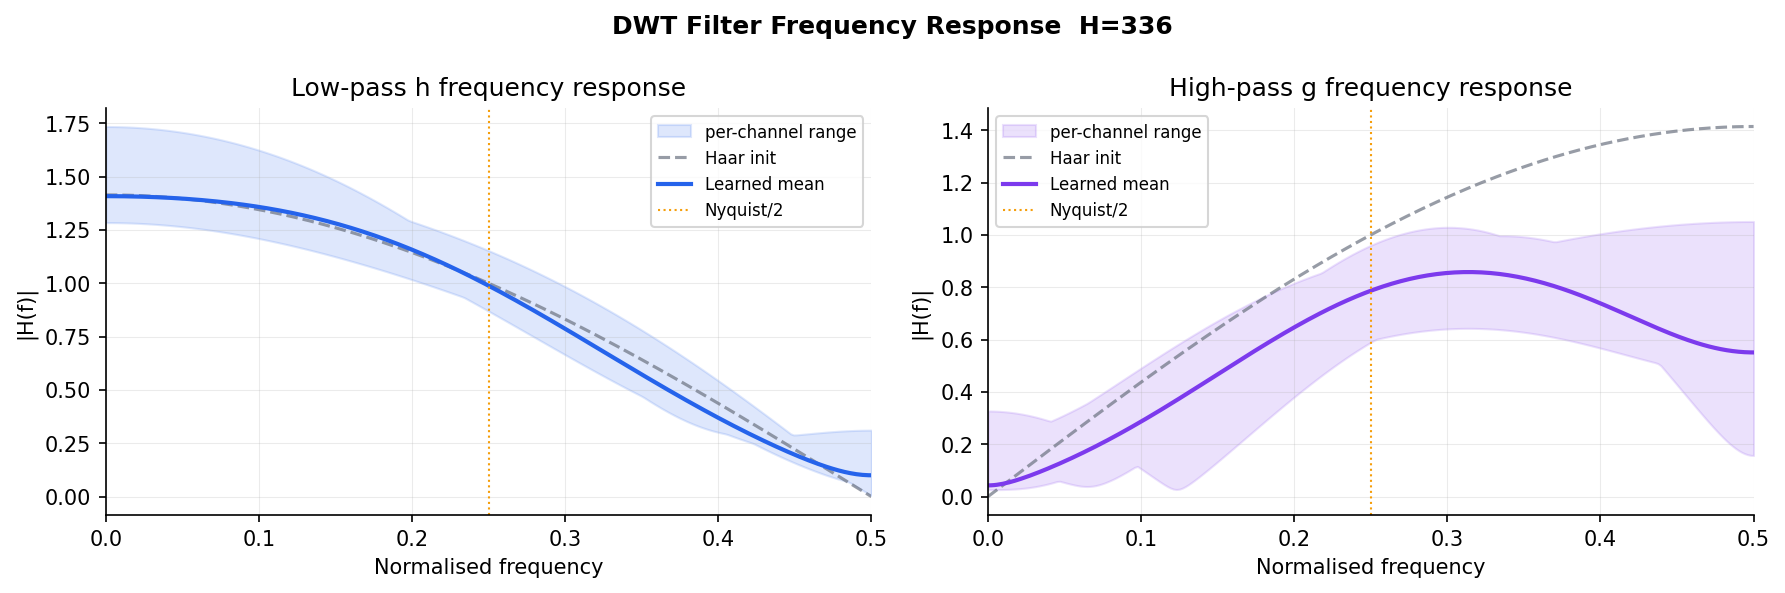
\includegraphics[width=0.49\linewidth]{plots-old/filters/H336_filter_spectrum.png}
  \\[4pt]
  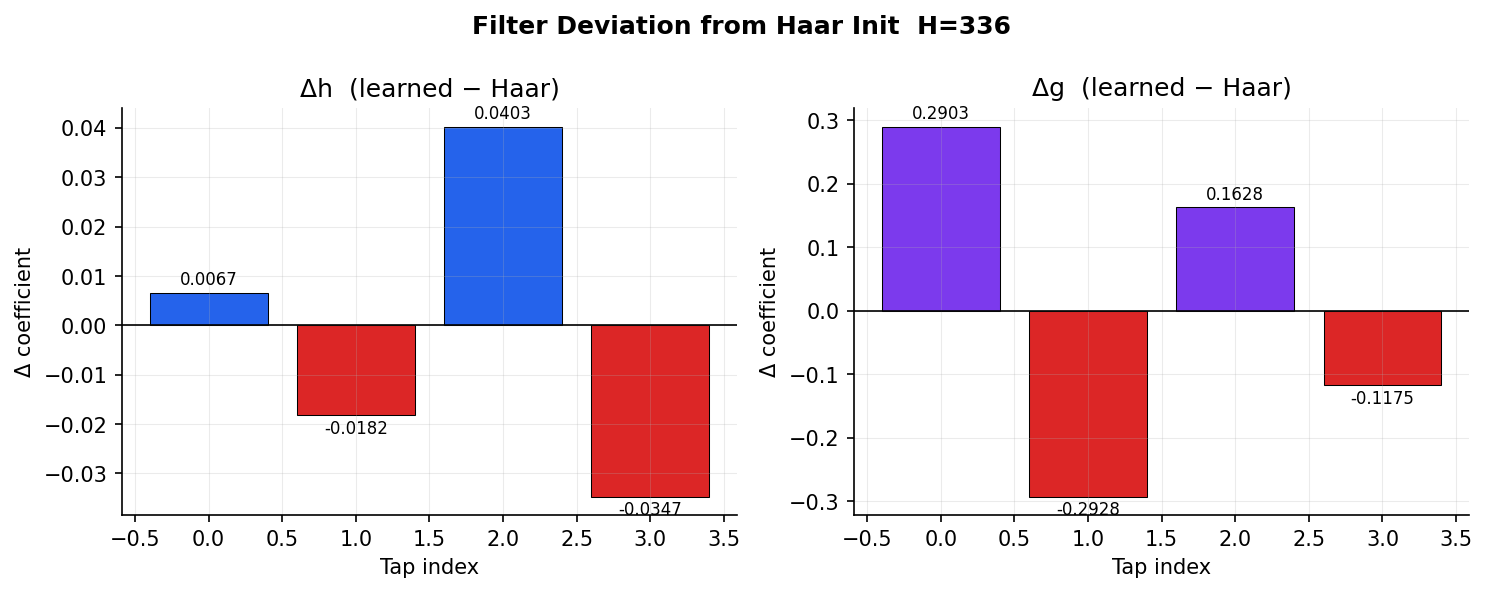
\includegraphics[width=0.49\linewidth]{plots-old/filters/H336_filter_evolution.png}
  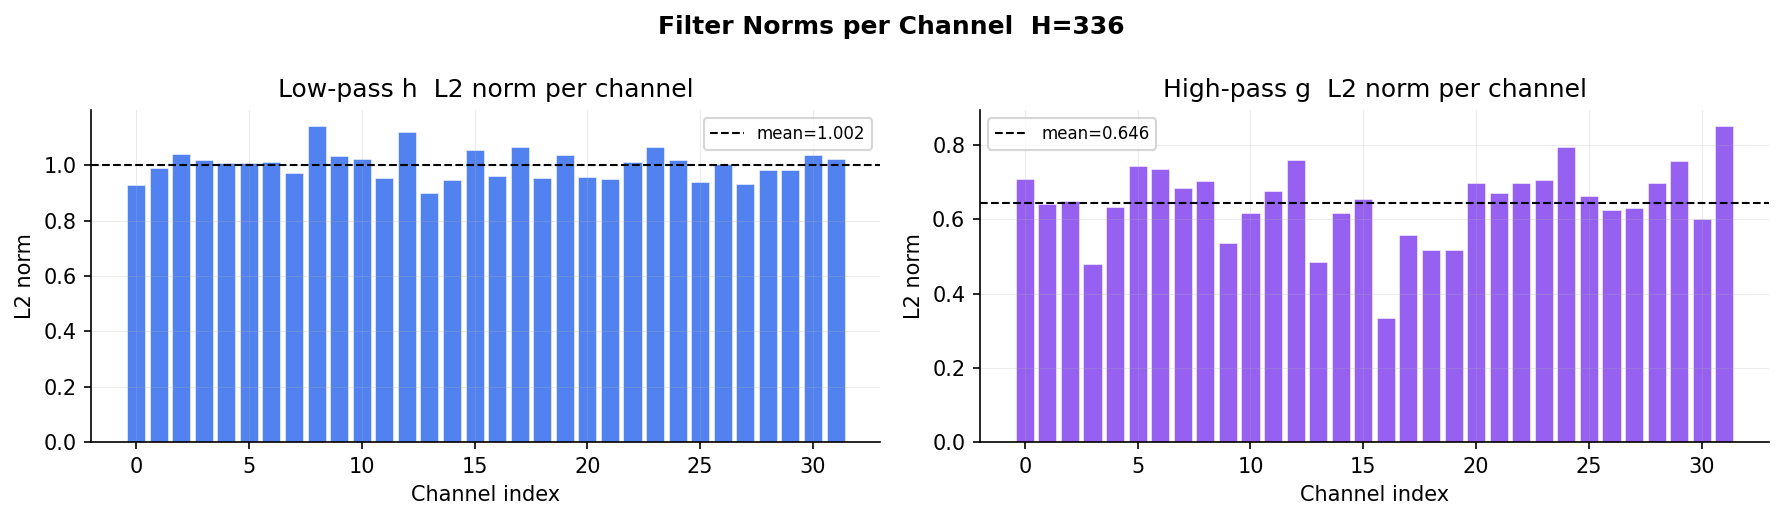
\includegraphics[width=0.49\linewidth]{plots-old/filters/H336_filter_stats.png}
  \caption{DWT filter analysis at $H=336$.}
  \label{fig:dwt-filters-336}
\end{figure}

\begin{figure}[H]
  \centering
  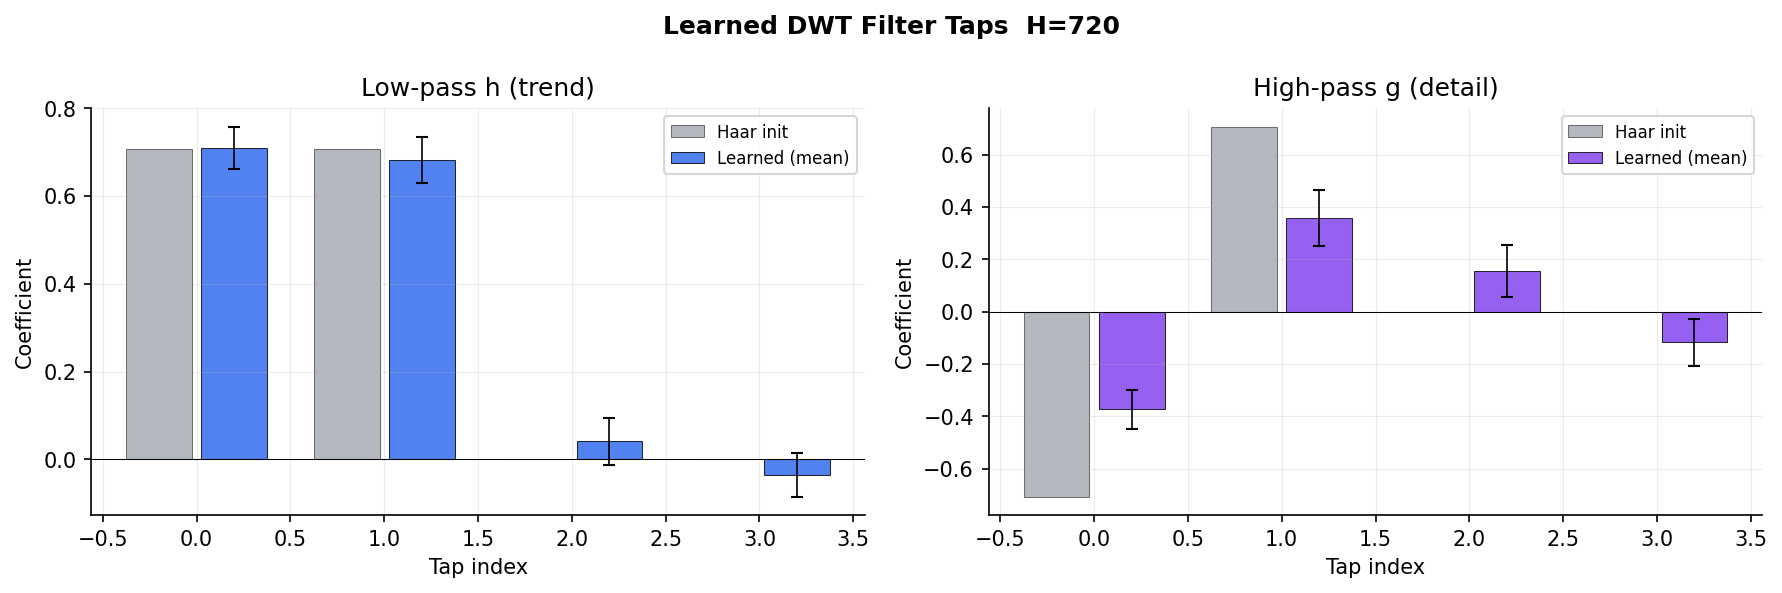
\includegraphics[width=0.49\linewidth]{plots-old/filters/H720_dwt_filters.png}
  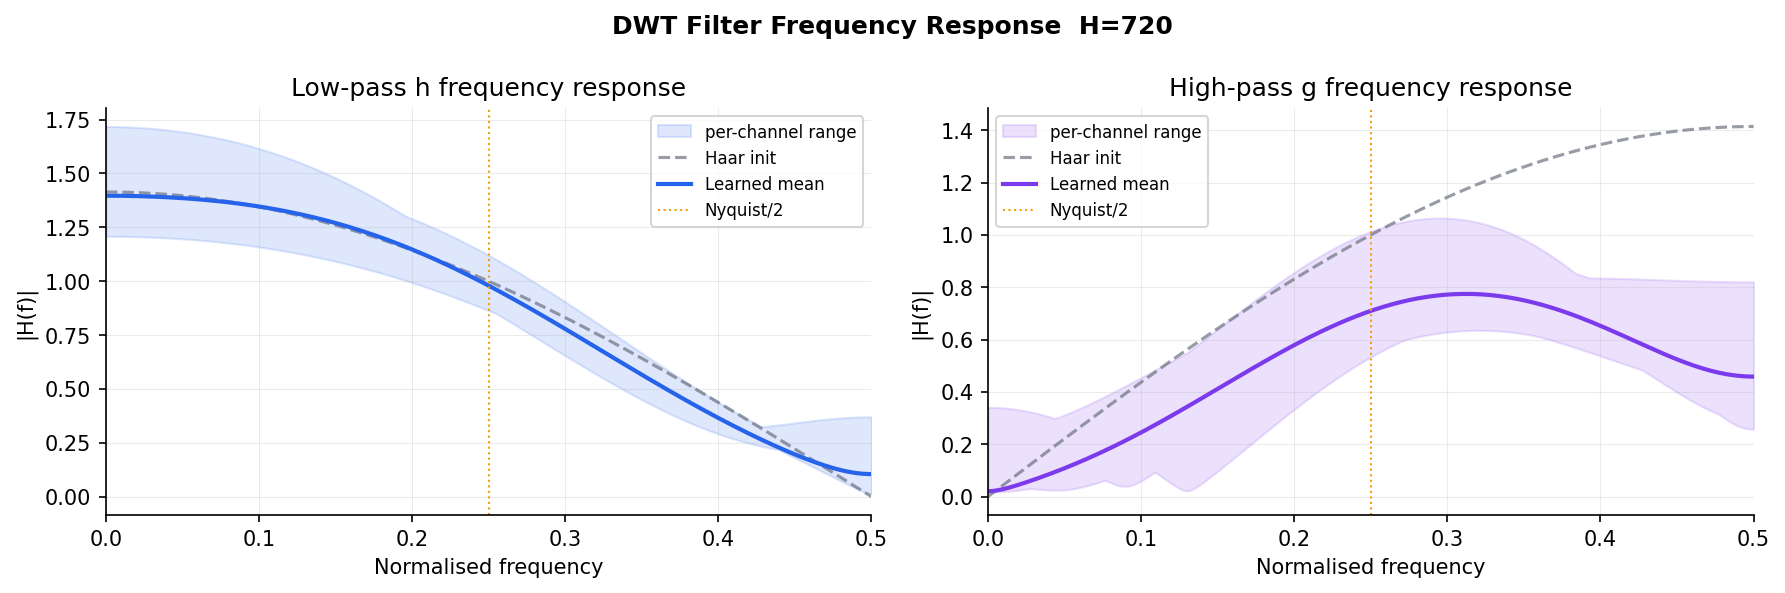
\includegraphics[width=0.49\linewidth]{plots-old/filters/H720_filter_spectrum.png}
  \\[4pt]
  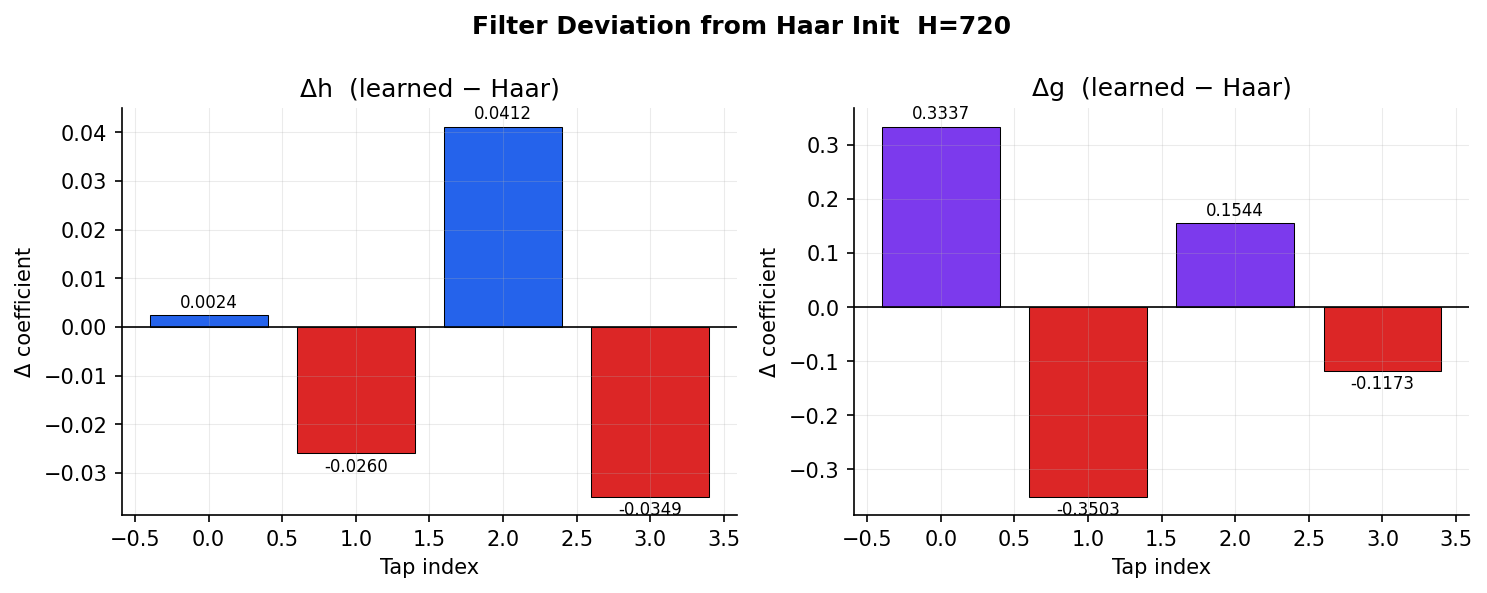
\includegraphics[width=0.49\linewidth]{plots-old/filters/H720_filter_evolution.png}
  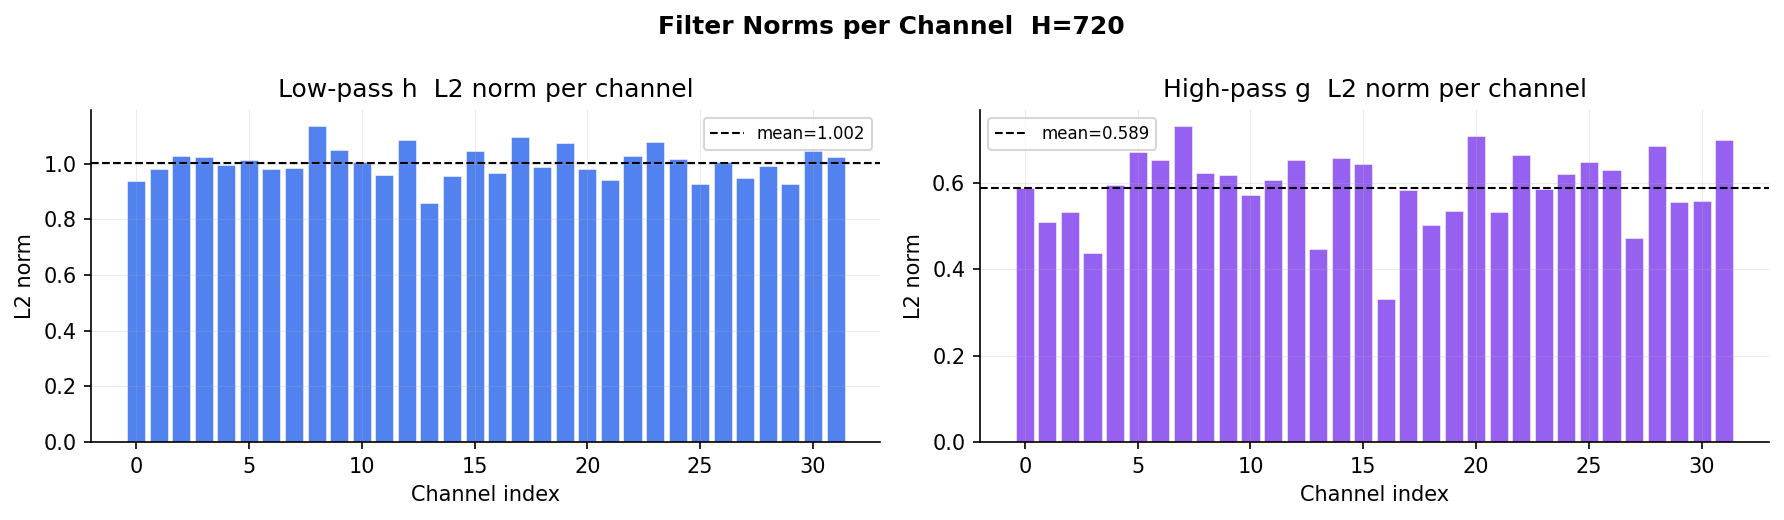
\includegraphics[width=0.49\linewidth]{plots-old/filters/H720_filter_stats.png}
  \caption{DWT filter analysis at $H=720$. At longer horizons the high-pass filter shows greater deviation from Haar, consistent with the need to suppress higher-frequency noise as prediction uncertainty grows.}
  \label{fig:dwt-filters-720}
\end{figure}

\begin{figure}[H]
  \centering
  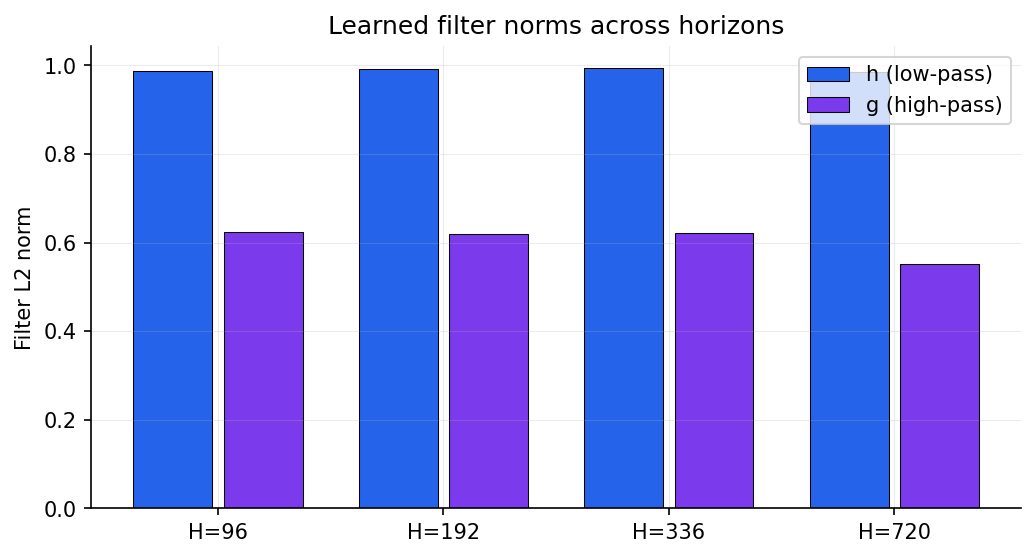
\includegraphics[width=\linewidth]{plots-old/filters/all_horizons_filter_norms.png}
  \caption{All-horizon comparison of per-channel L2 filter norms. The consistent ordering across horizons suggests that filter adaptation is horizon-agnostic at the per-channel level.}
  \label{fig:filter-norms-all}
\end{figure}

\subsection{Spectral Analysis}

Figure~\ref{fig:spectral-96} presents the spectral analysis at $H=96$: time-domain and frequency-domain plots comparing the prediction PSD against the target PSD. The spectral penalty visibly aligns the prediction PSD with the target, mitigating the over-smoothing effect otherwise induced by MSE-only training.

\begin{figure}[H]
  \centering
  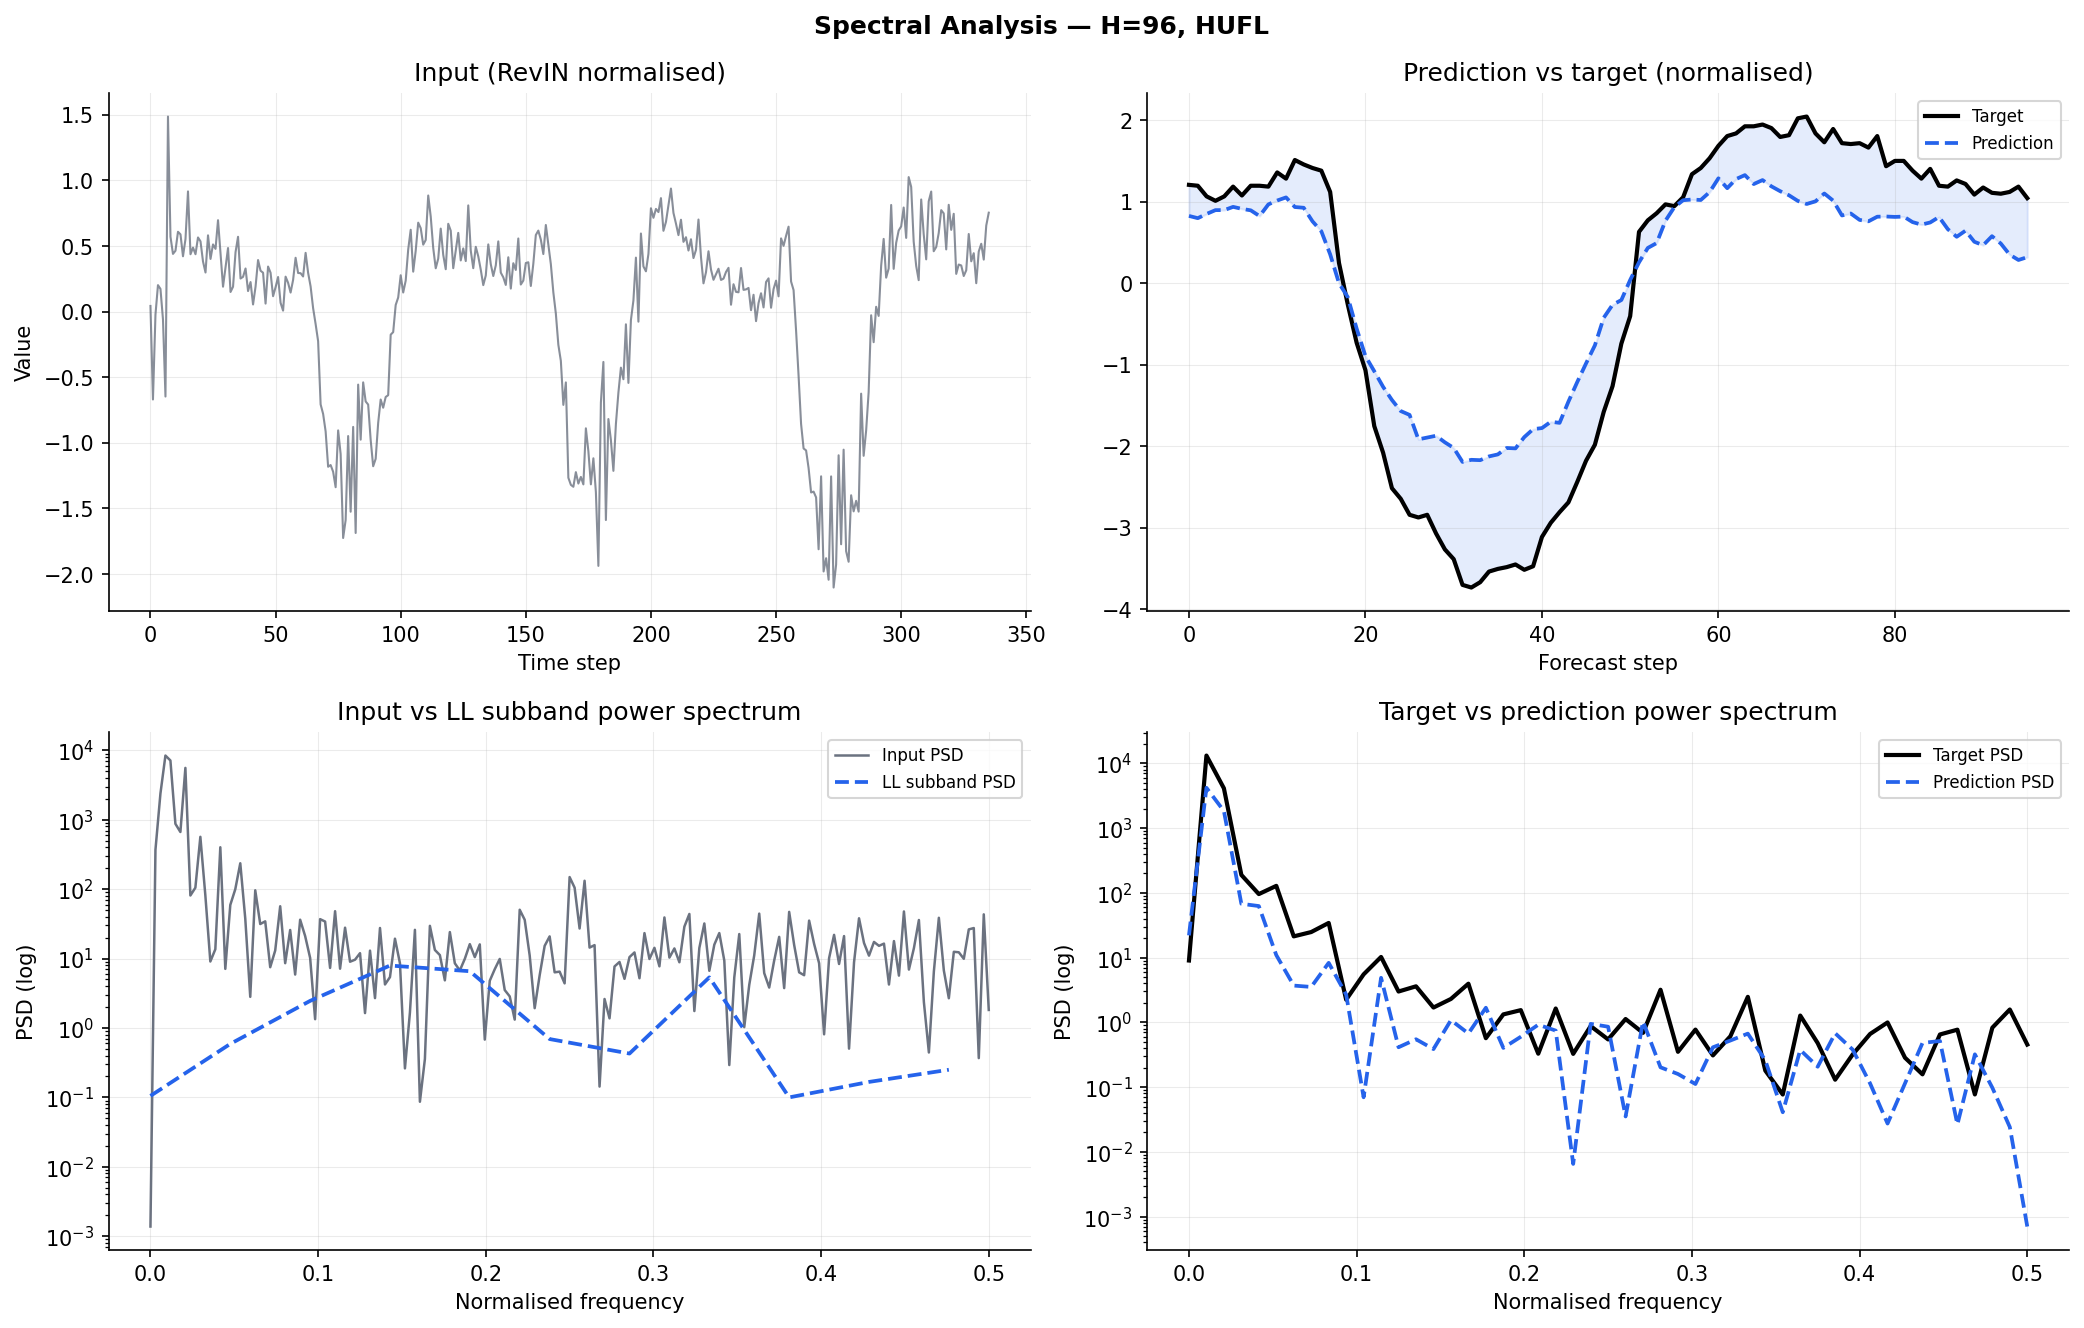
\includegraphics[width=\linewidth]{plots-old/benchmarks/H96_spectral.png}
  \caption{Spectral analysis at $H=96$. Top row: time-domain prediction vs.\ target. Bottom row: power spectral density — input vs.\ LL subband (left), and prediction vs.\ target (right).}
  \label{fig:spectral-96}
\end{figure}

\begin{figure}[H]
  \centering
  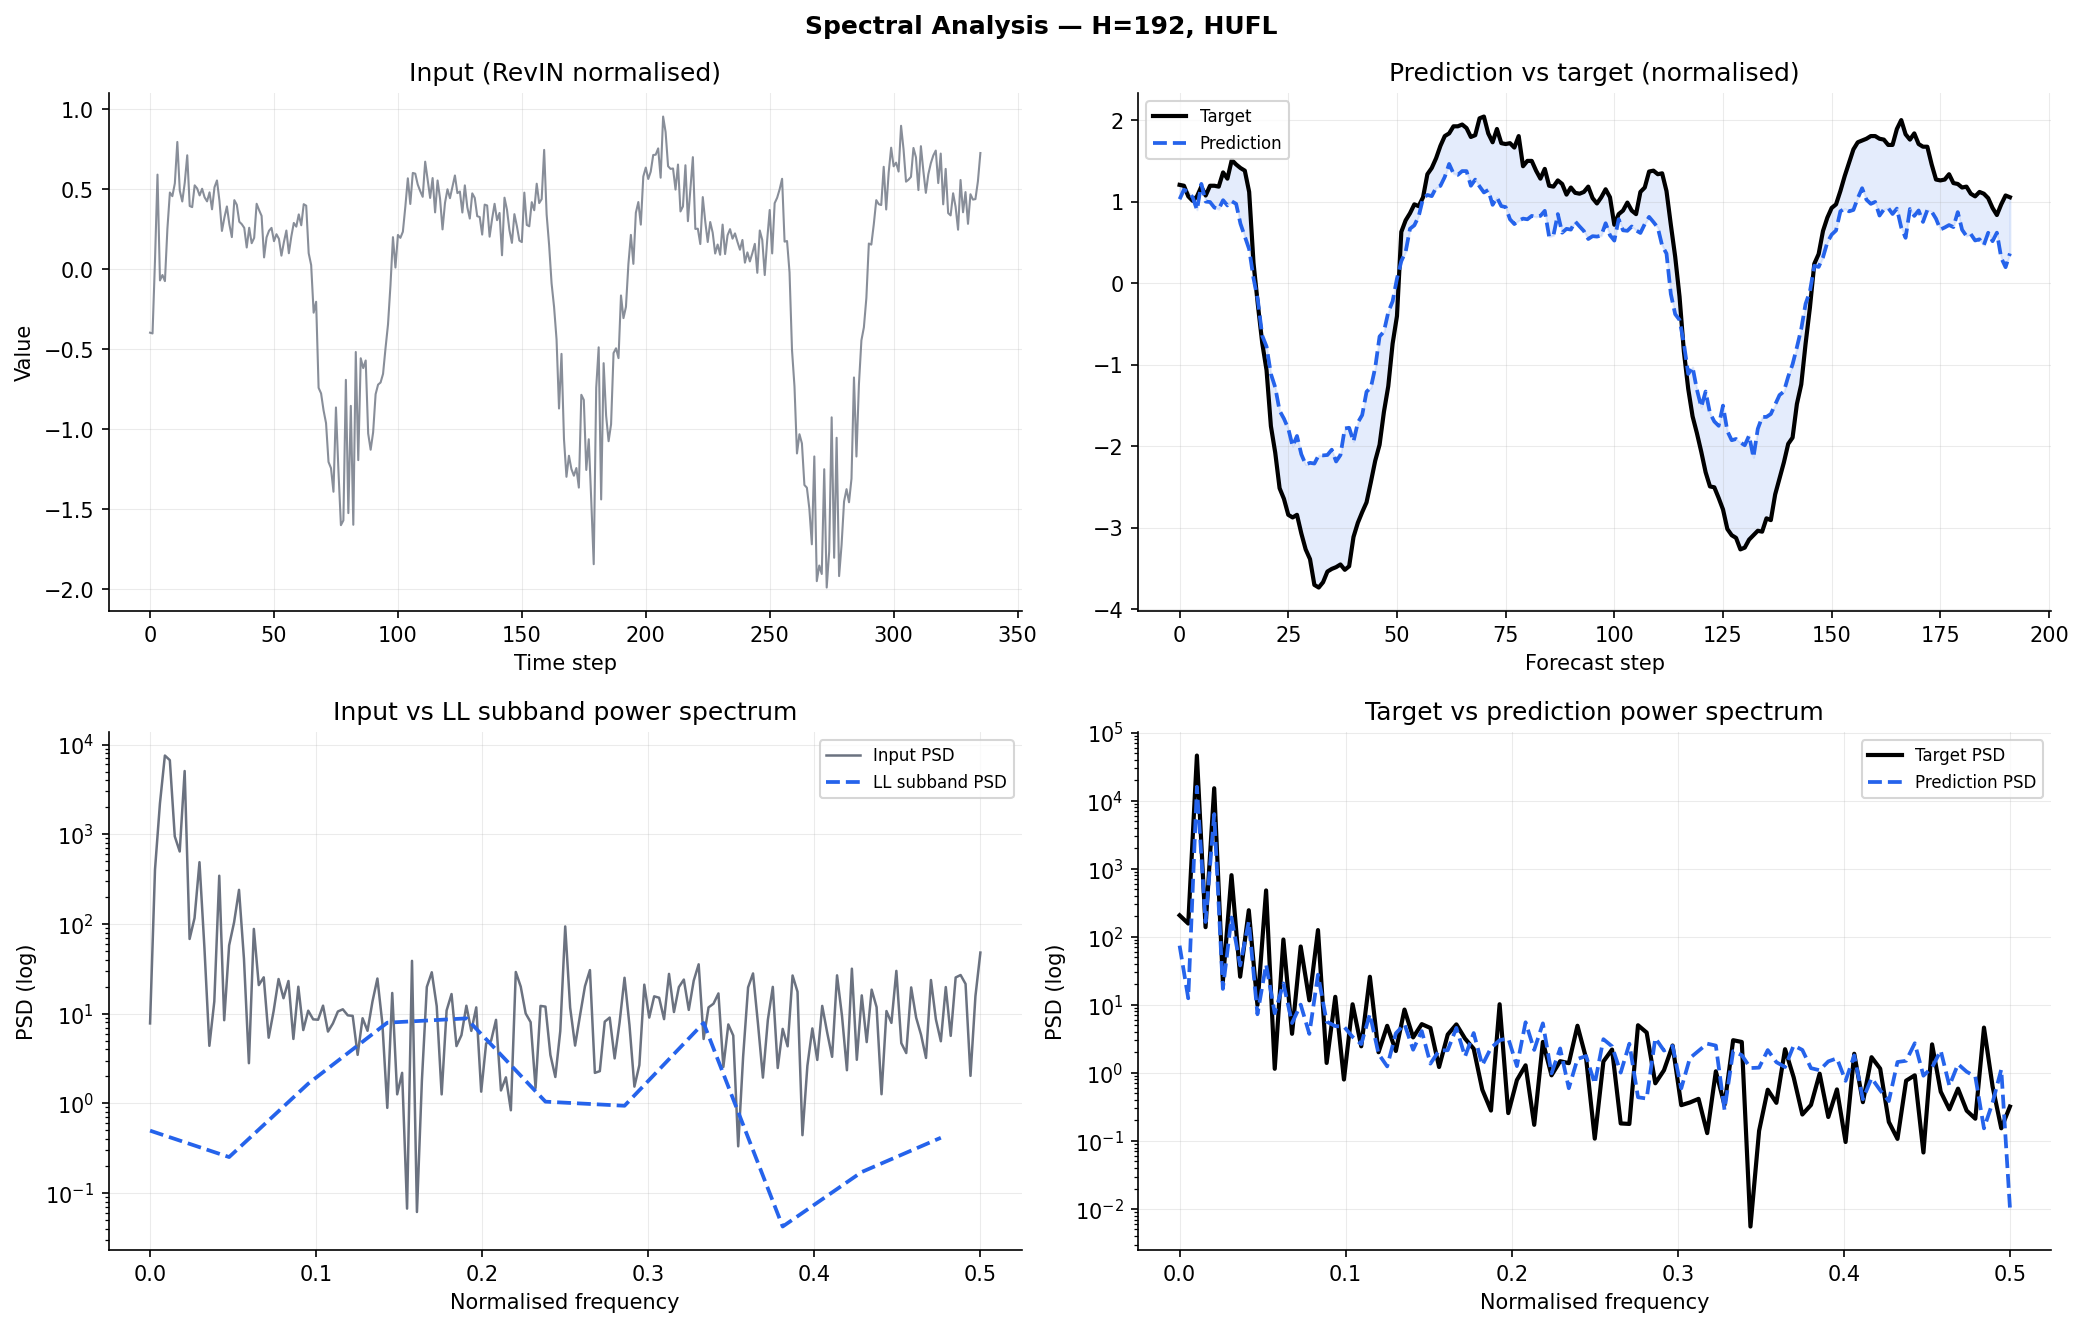
\includegraphics[width=0.49\linewidth]{plots-old/benchmarks/H192_spectral.png}
  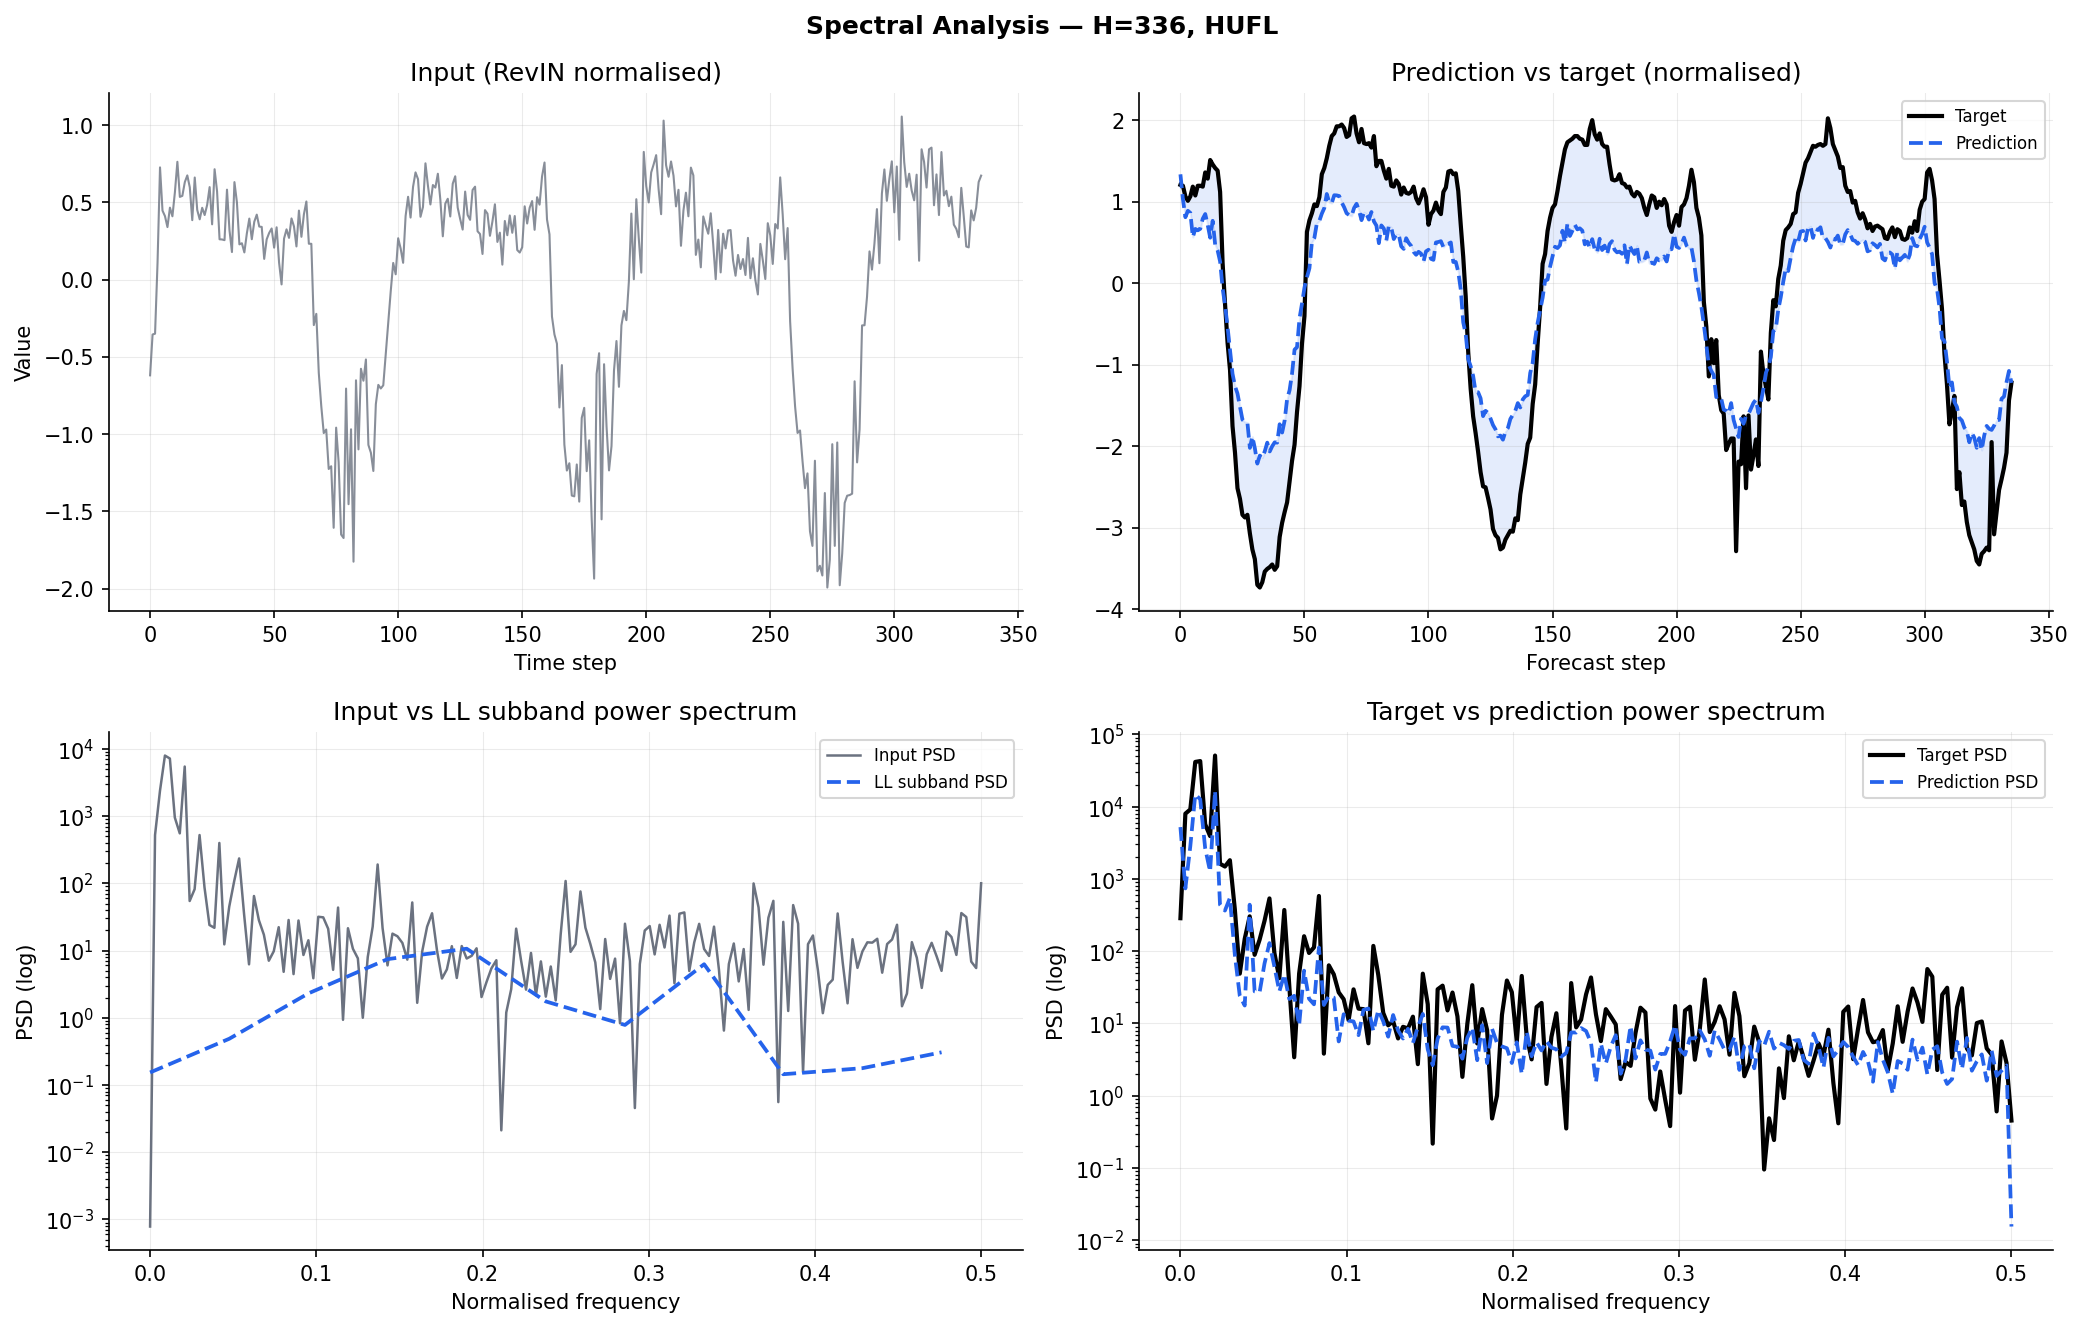
\includegraphics[width=0.49\linewidth]{plots-old/benchmarks/H336_spectral.png}
  \\[6pt]
  \centering
  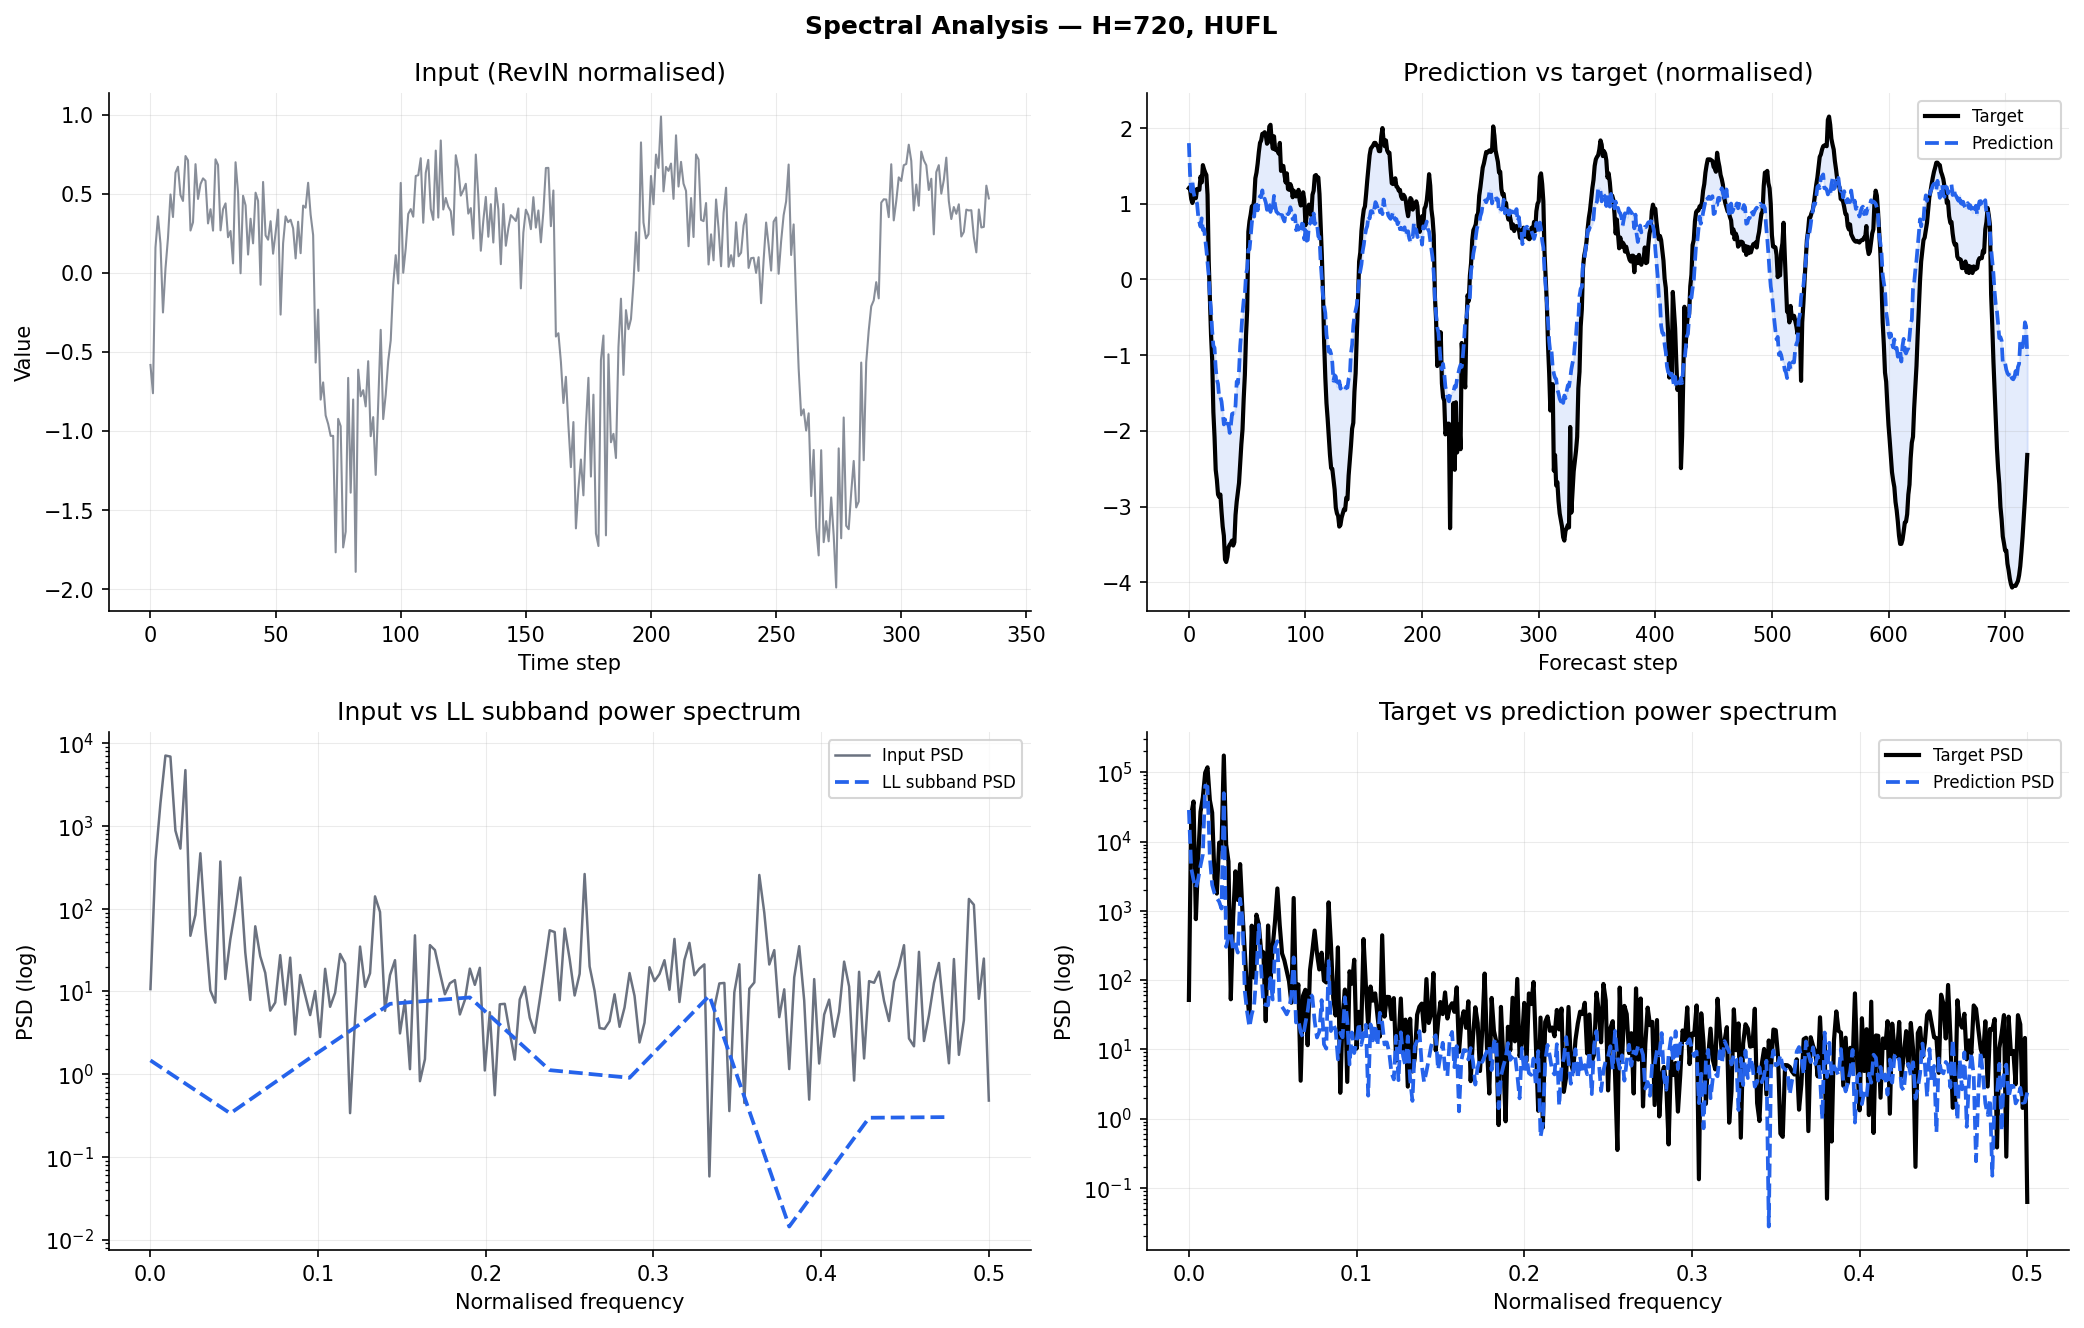
\includegraphics[width=0.49\linewidth]{plots-old/benchmarks/H720_spectral.png}
  \caption{Spectral analysis at $H \in \{192, 336, 720\}$. PSD alignment between prediction and target remains consistent across horizons, indicating robust spectral regularisation.}
  \label{fig:spectral-others}
\end{figure}

\subsection{Attention Analysis}

Figure~\ref{fig:attention-96} shows the LL-subband attention weight matrix (heads averaged) and the learned sparsity threshold $\tau$ for the high-frequency routing path at $H=96$. The attention maps reveal diagonal-dominant structure with moderate off-diagonal mass, indicating that the model primarily attends to local patches while retaining some global context. The threshold $\tau$ is learned to be non-trivially positive, confirming that sparse gating is active.

\begin{figure}[H]
  \centering
  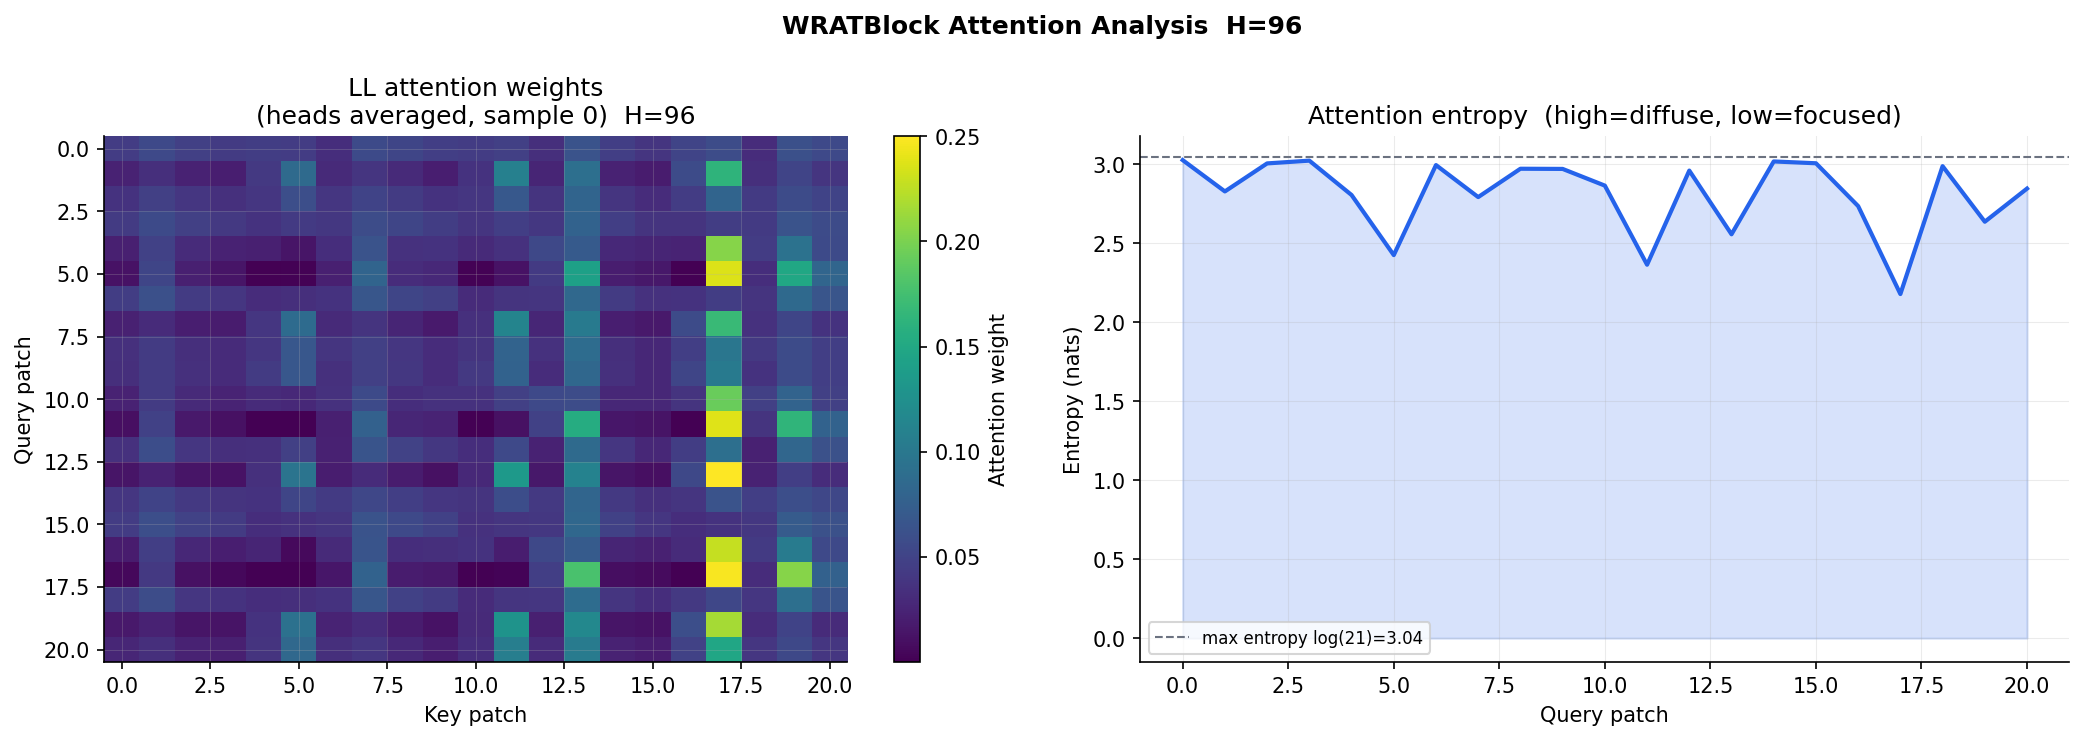
\includegraphics[width=0.49\linewidth]{plots-old/attention/H96_wrat_attn.png}
  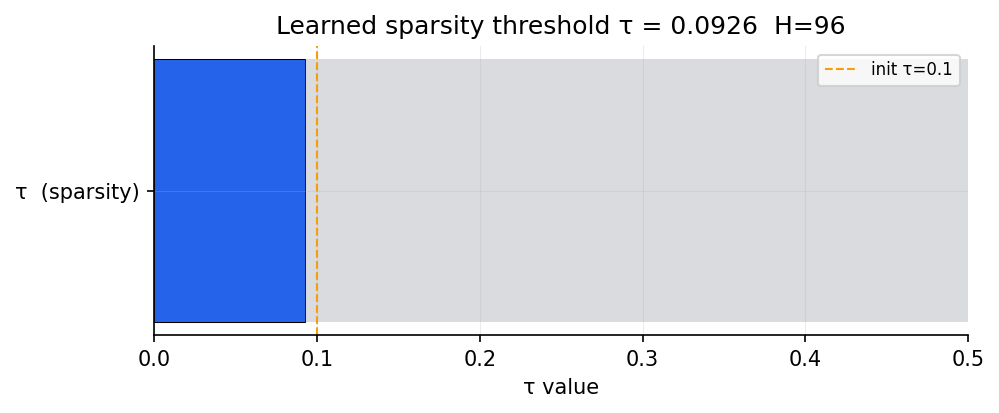
\includegraphics[width=0.49\linewidth]{plots-old/attention/H96_tau_bar.png}
  \caption{$H=96$. Left: LL-subband attention weight matrix (heads averaged). Right: Learned sparsity threshold $\tau$ for the HF routing path.}
  \label{fig:attention-96}
\end{figure}

\begin{figure}[H]
  \centering
  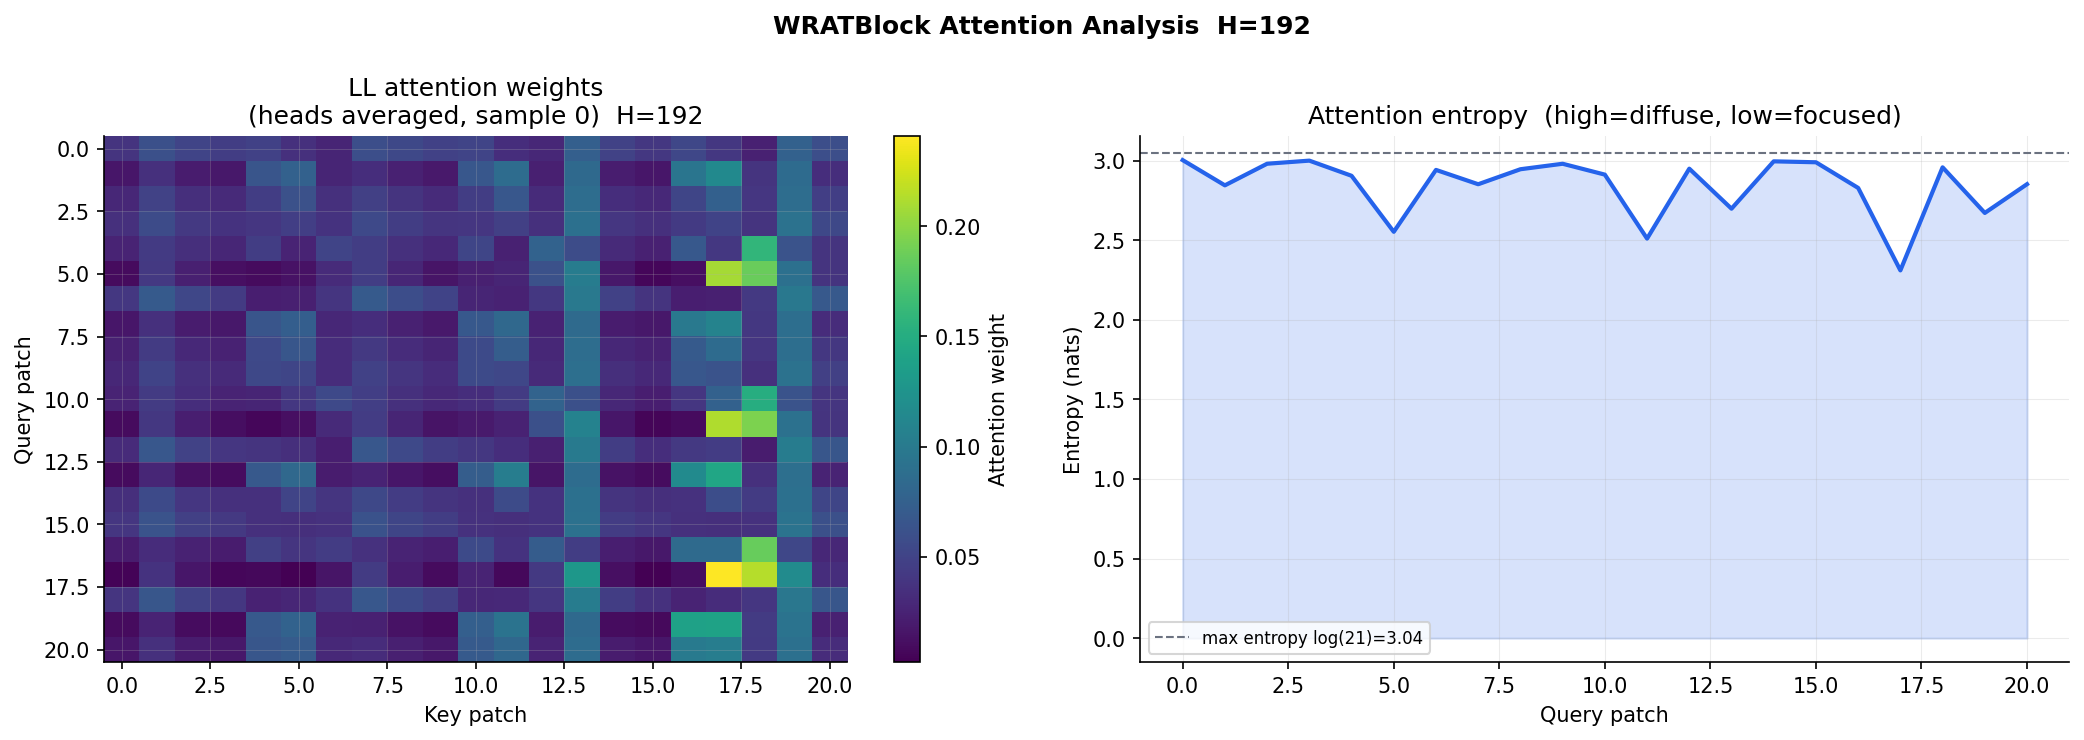
\includegraphics[width=0.49\linewidth]{plots-old/attention/H192_wrat_attn.png}
  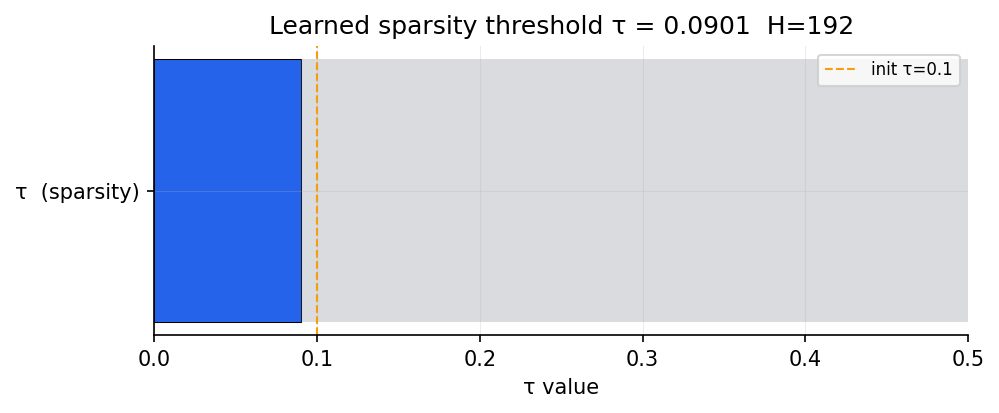
\includegraphics[width=0.49\linewidth]{plots-old/attention/H192_tau_bar.png}
  \caption{Attention analysis at $H=192$.}
  \label{fig:attention-192}
\end{figure}

\begin{figure}[H]
  \centering
  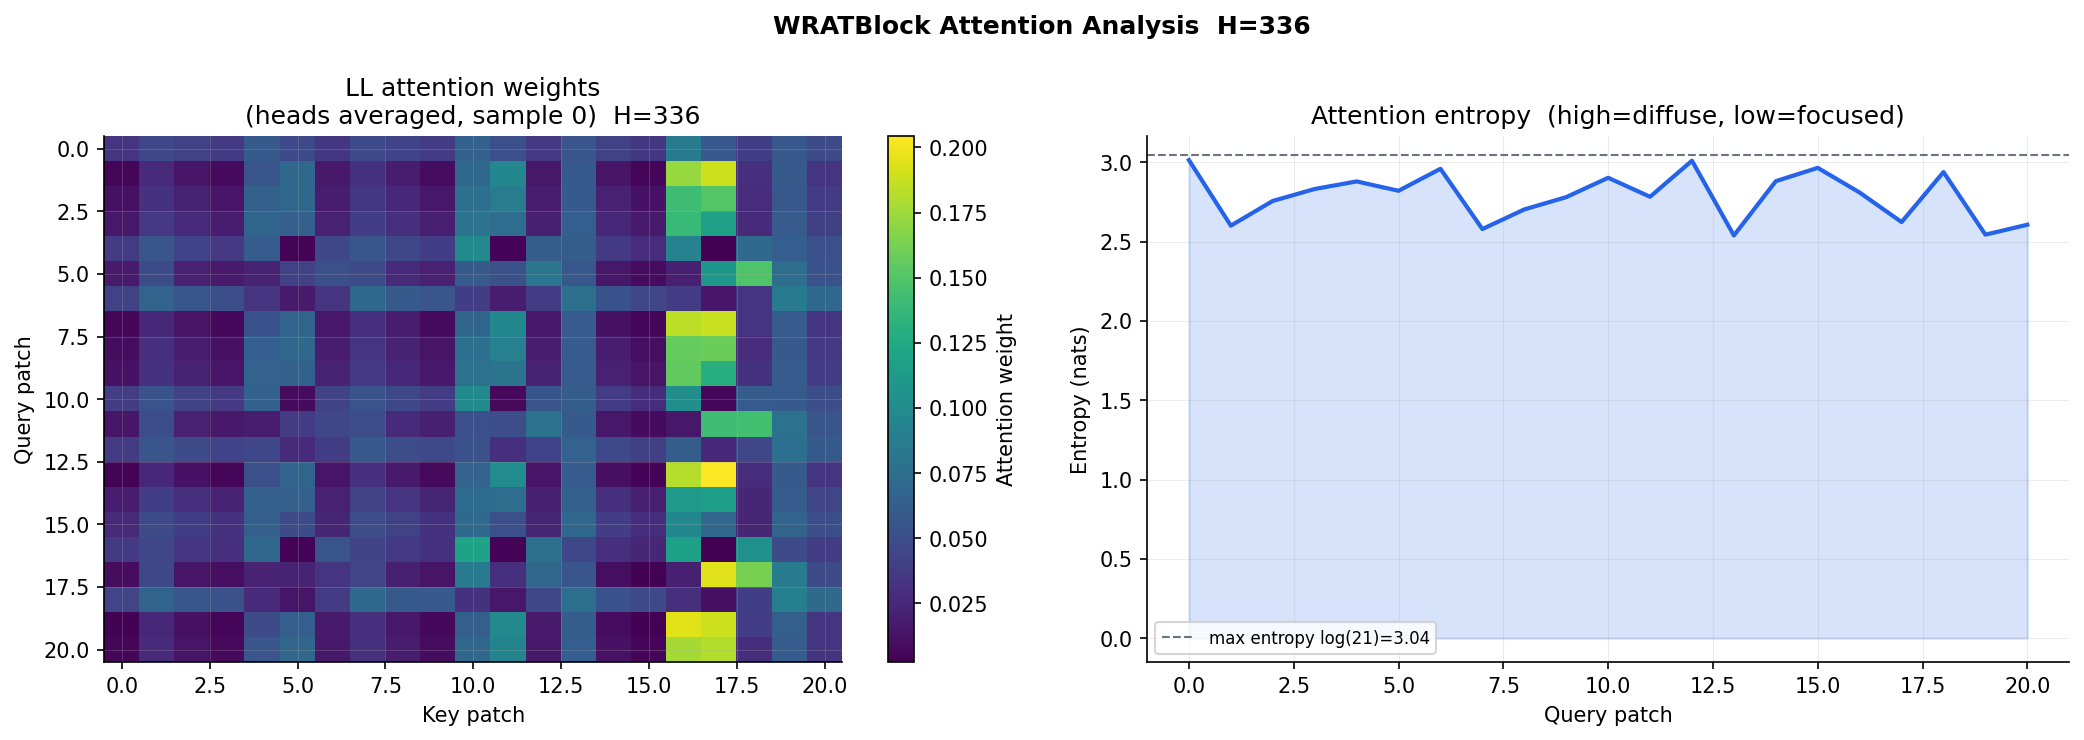
\includegraphics[width=0.49\linewidth]{plots-old/attention/H336_wrat_attn.png}
  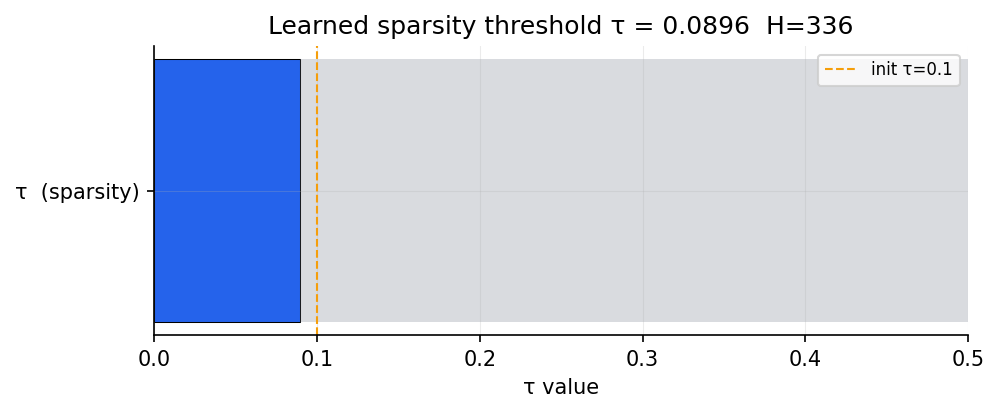
\includegraphics[width=0.49\linewidth]{plots-old/attention/H336_tau_bar.png}
  \caption{Attention analysis at $H=336$.}
  \label{fig:attention-336}
\end{figure}

\begin{figure}[H]
  \centering
  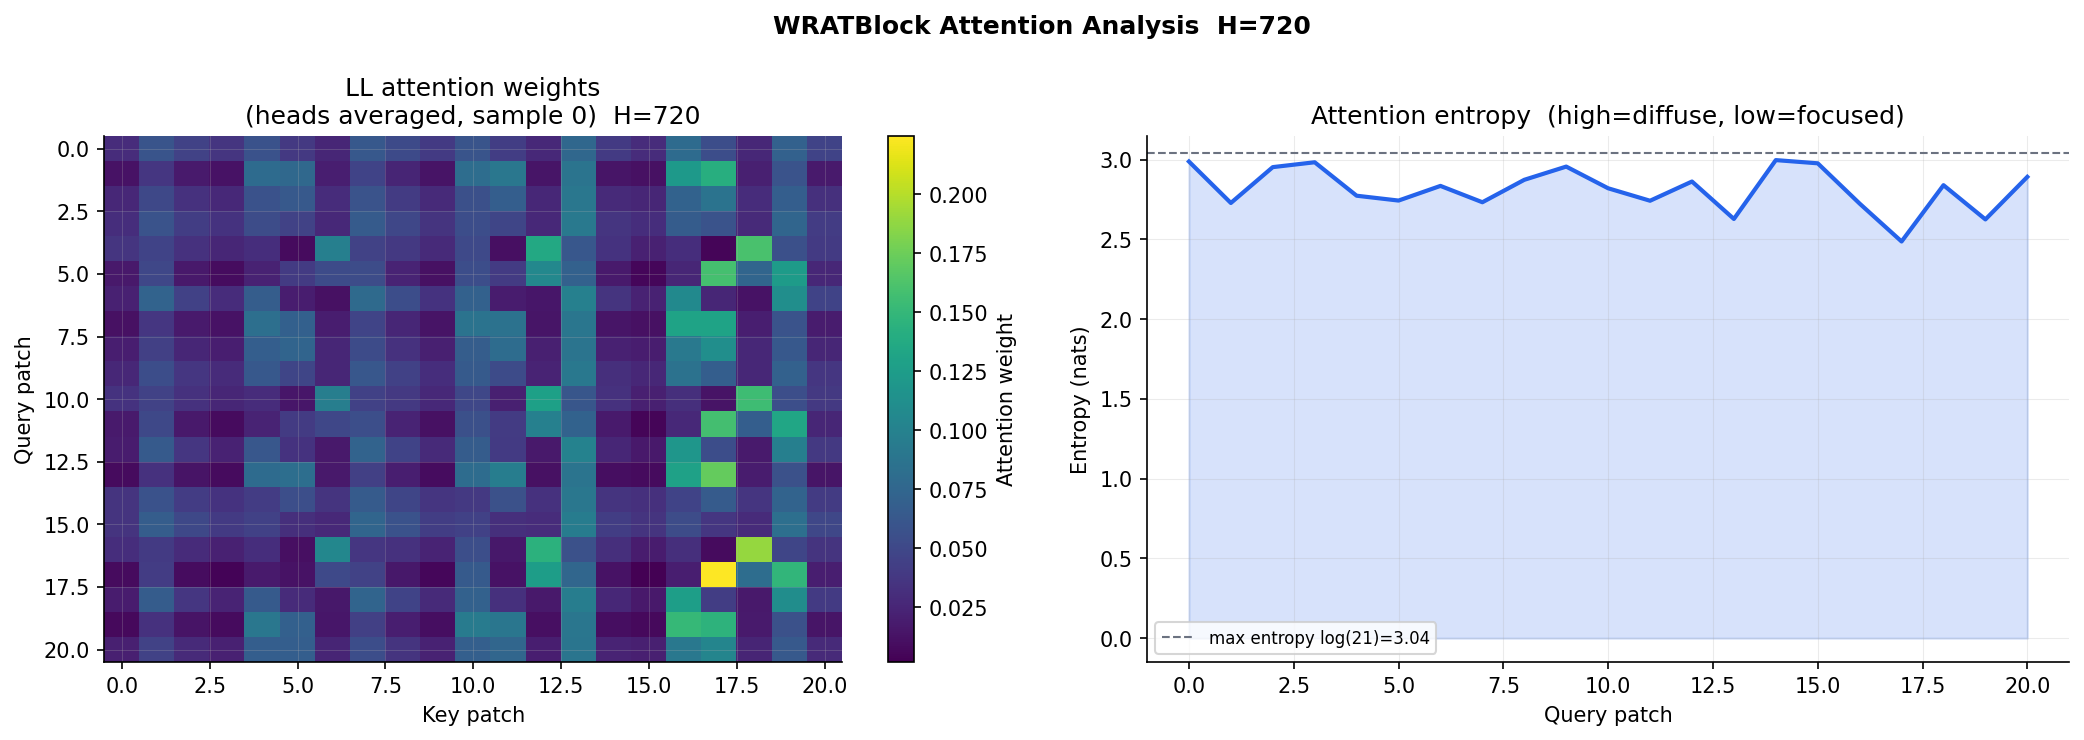
\includegraphics[width=0.49\linewidth]{plots-old/attention/H720_wrat_attn.png}
  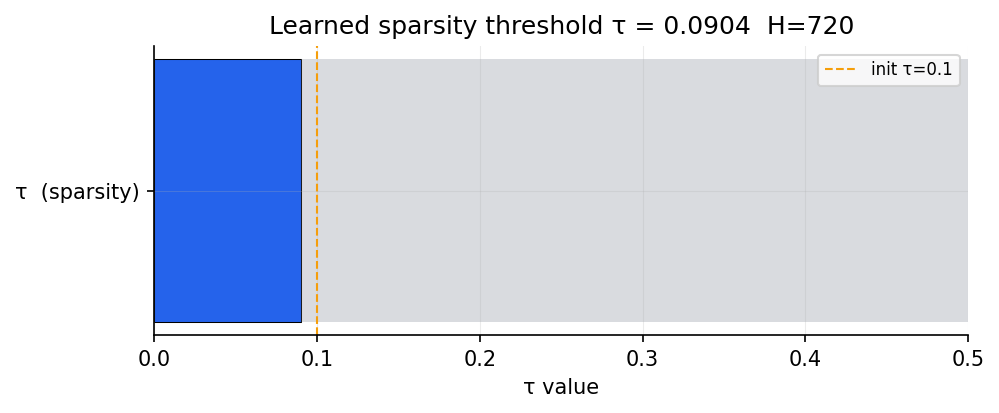
\includegraphics[width=0.49\linewidth]{plots-old/attention/H720_tau_bar.png}
  \caption{Attention analysis at $H=720$. The attention matrix becomes sparser at longer horizons, consistent with the model relying more on local context when long-range information is less reliable.}
  \label{fig:attention-720}
\end{figure}

\subsection{Variate Graph and Cross-Variate Attention}

Although P-WSA v8.0 operates under strict Channel Independence, we record cross-variate attention statistics as a diagnostic tool to understand latent correlations in the data that the model implicitly exploits via shared weights.

\begin{figure}[H]
  \centering
  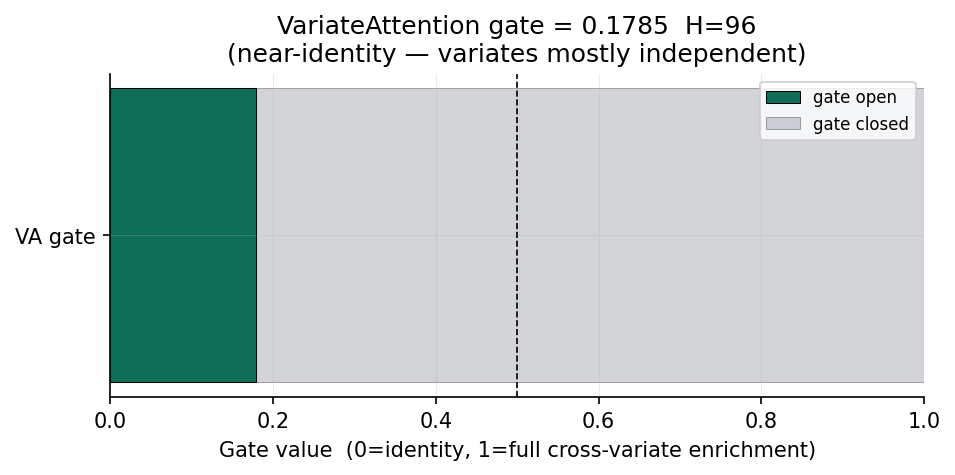
\includegraphics[width=0.49\linewidth]{plots-old/variate_graph/H96_variate_attn.png}
  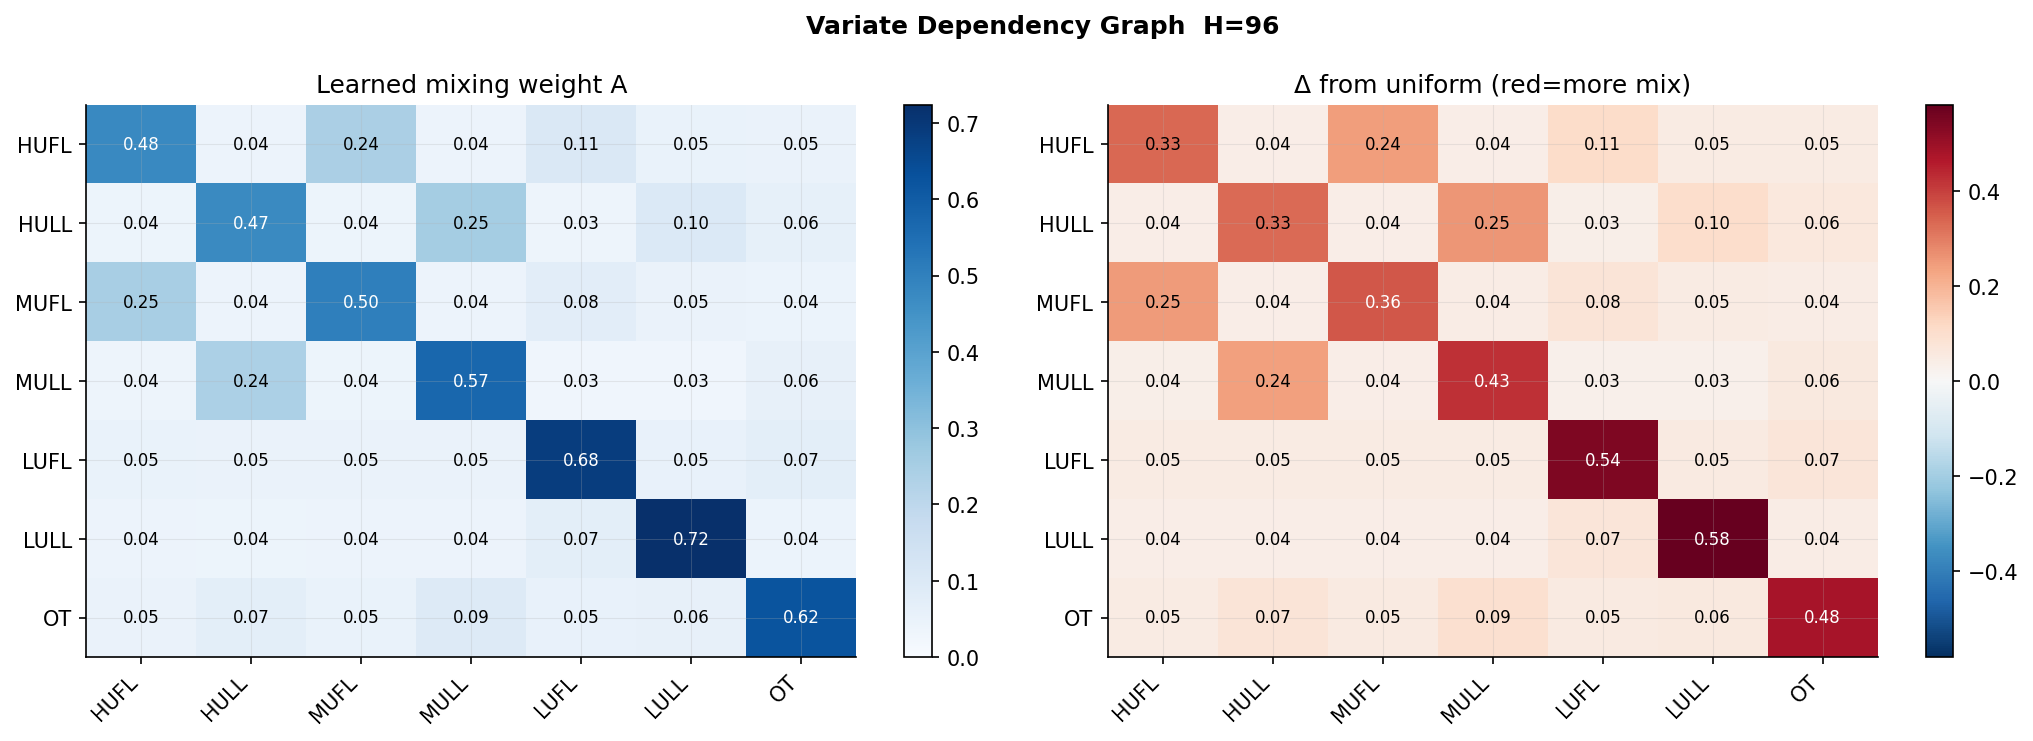
\includegraphics[width=0.49\linewidth]{plots-old/variate_graph/H96_adjacency.png}
  \caption{$H=96$. Left: Cross-variate attention heatmap. Right: Binarised adjacency matrix of the variate interaction graph.}
  \label{fig:variate-96}
\end{figure}

\begin{figure}[H]
  \centering
  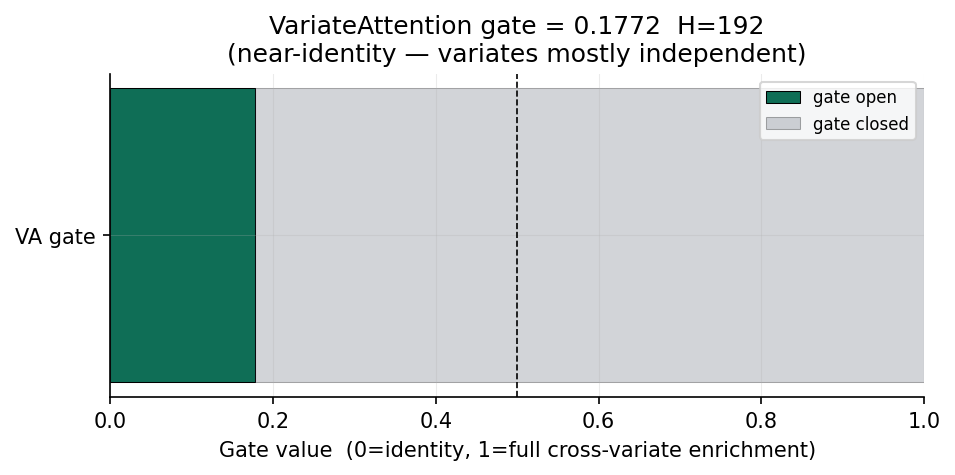
\includegraphics[width=0.49\linewidth]{plots-old/variate_graph/H192_variate_attn.png}
  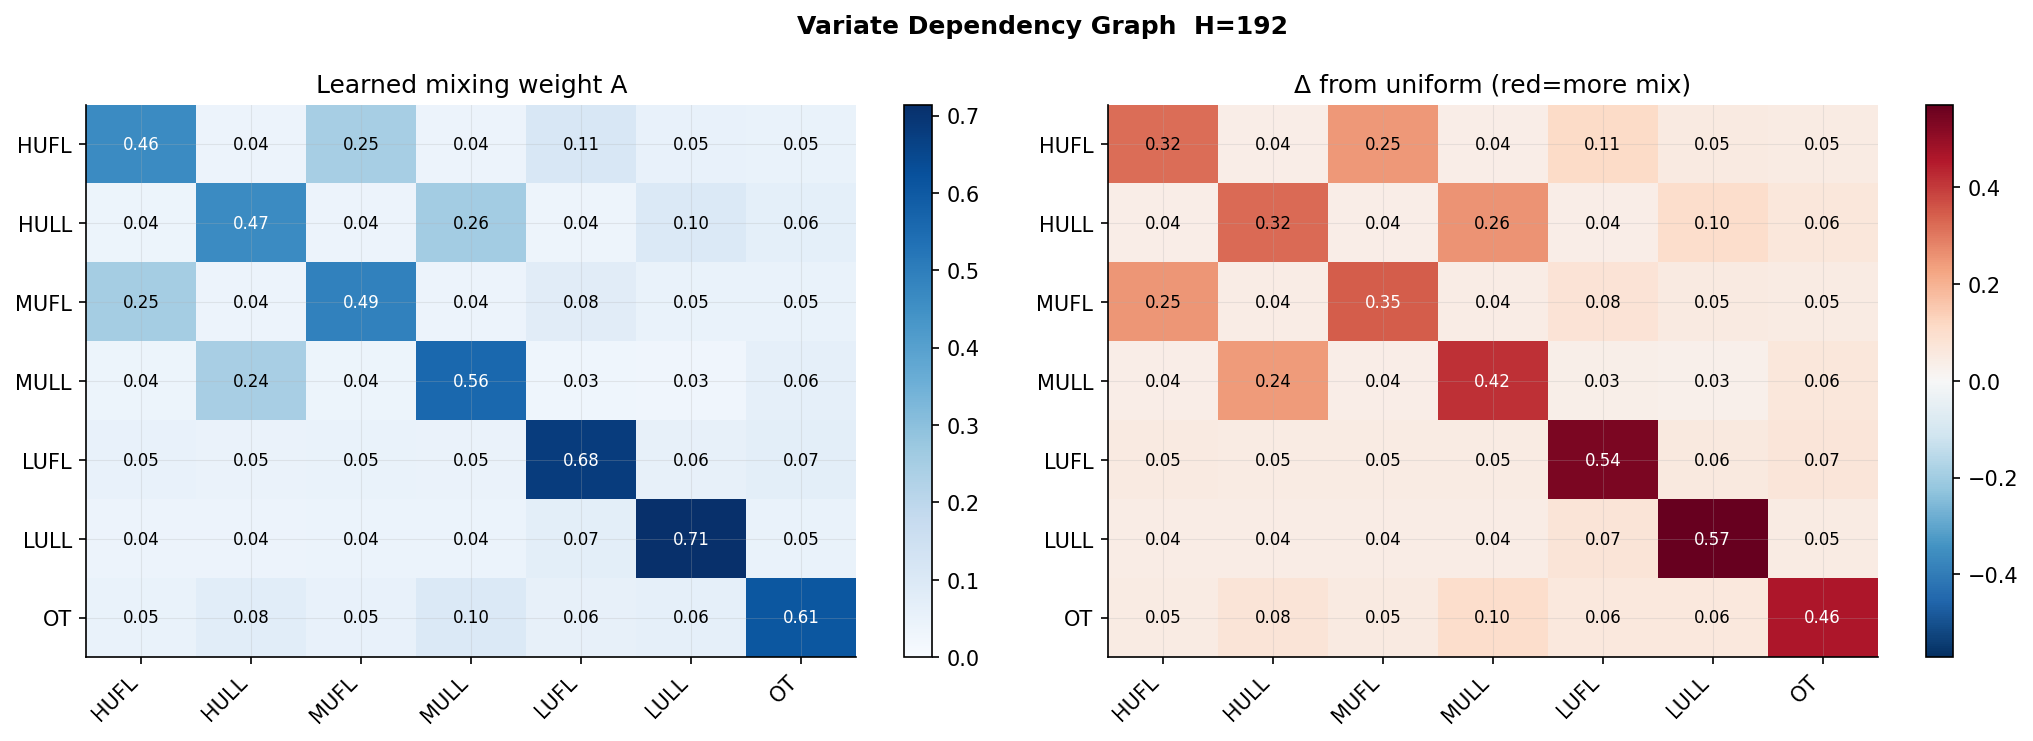
\includegraphics[width=0.49\linewidth]{plots-old/variate_graph/H192_adjacency.png}
  \caption{Variate graph analysis at $H=192$.}
  \label{fig:variate-192}
\end{figure}

\begin{figure}[H]
  \centering
  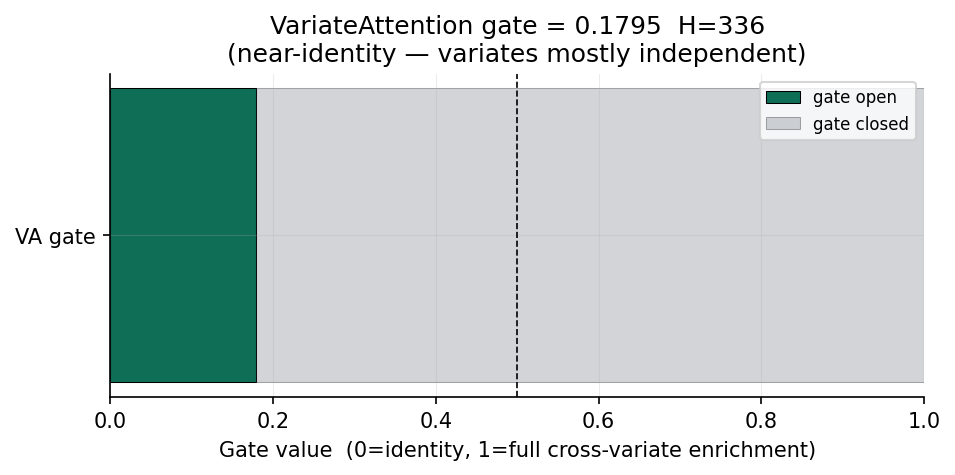
\includegraphics[width=0.49\linewidth]{plots-old/variate_graph/H336_variate_attn.png}
  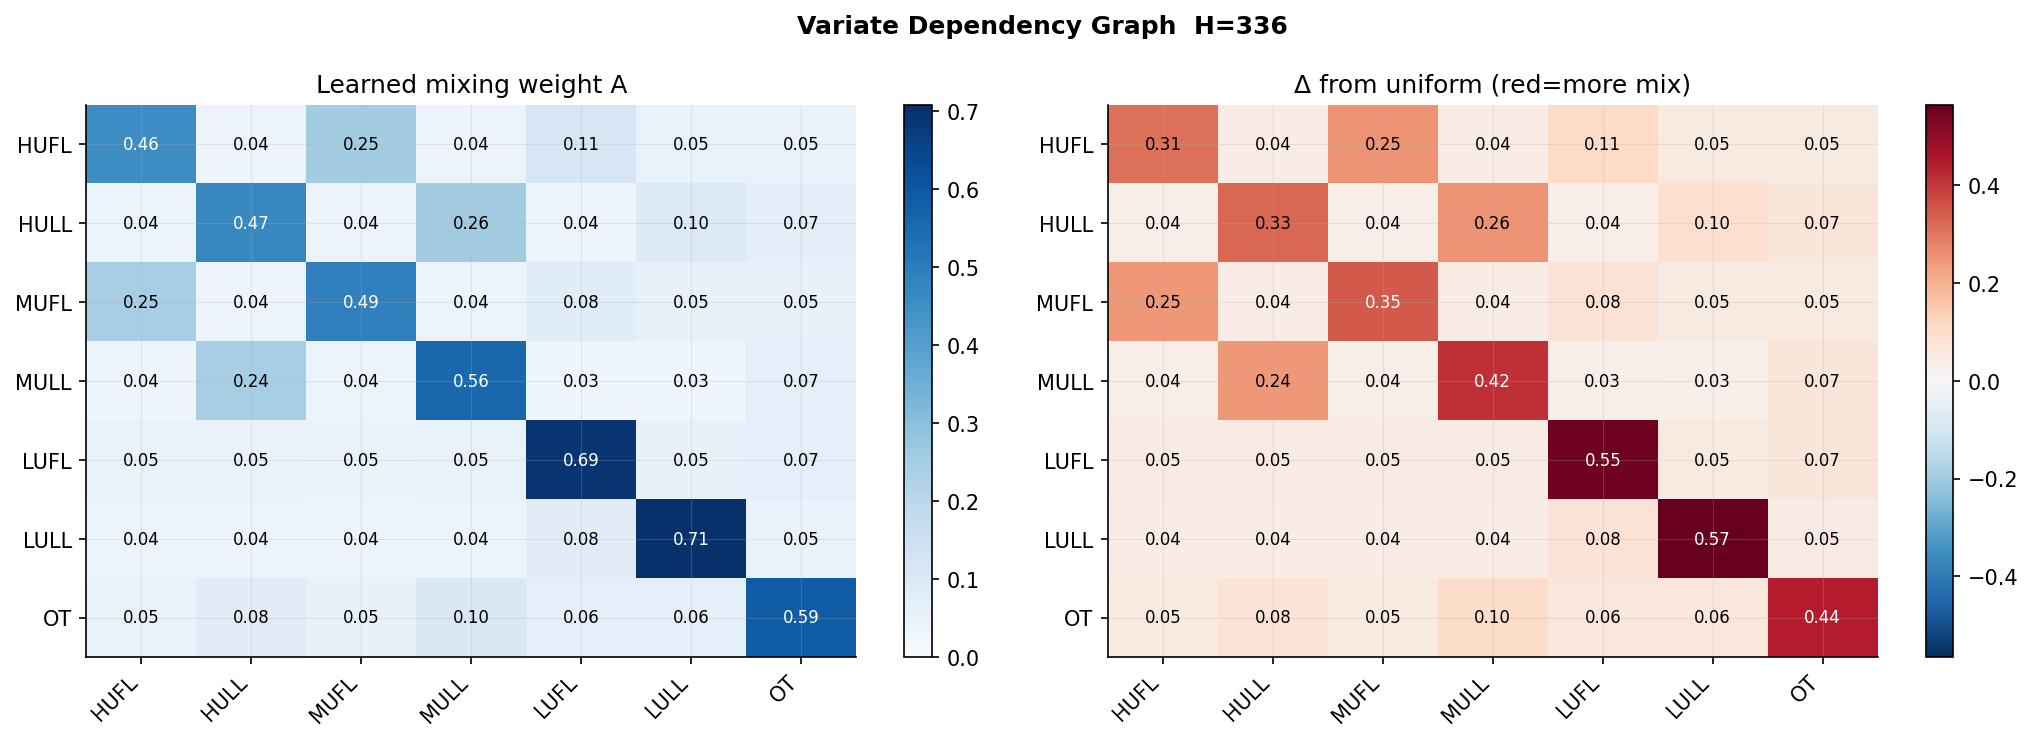
\includegraphics[width=0.49\linewidth]{plots-old/variate_graph/H336_adjacency.png}
  \caption{Variate graph analysis at $H=336$.}
  \label{fig:variate-336}
\end{figure}

\begin{figure}[H]
  \centering
  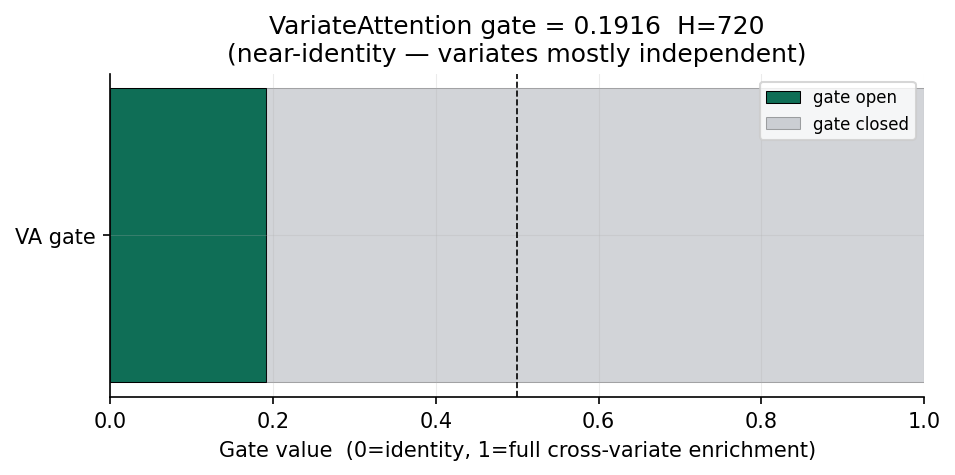
\includegraphics[width=0.49\linewidth]{plots-old/variate_graph/H720_variate_attn.png}
  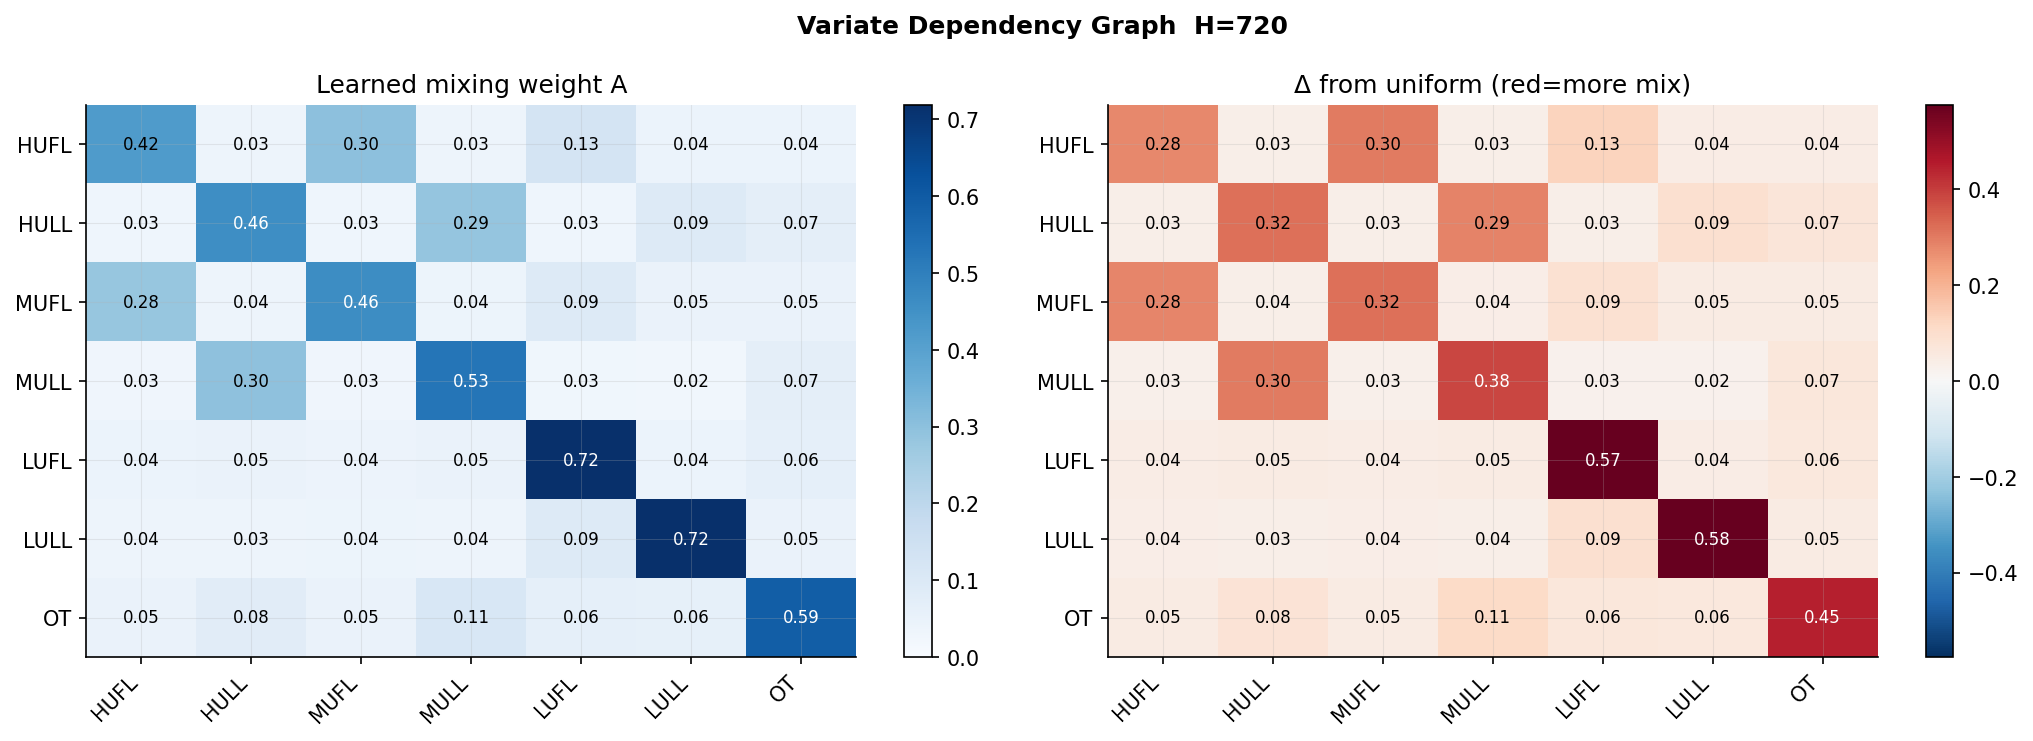
\includegraphics[width=0.49\linewidth]{plots-old/variate_graph/H720_adjacency.png}
  \caption{Variate graph analysis at $H=720$.}
  \label{fig:variate-720}
\end{figure}

\begin{figure}[H]
  \centering
  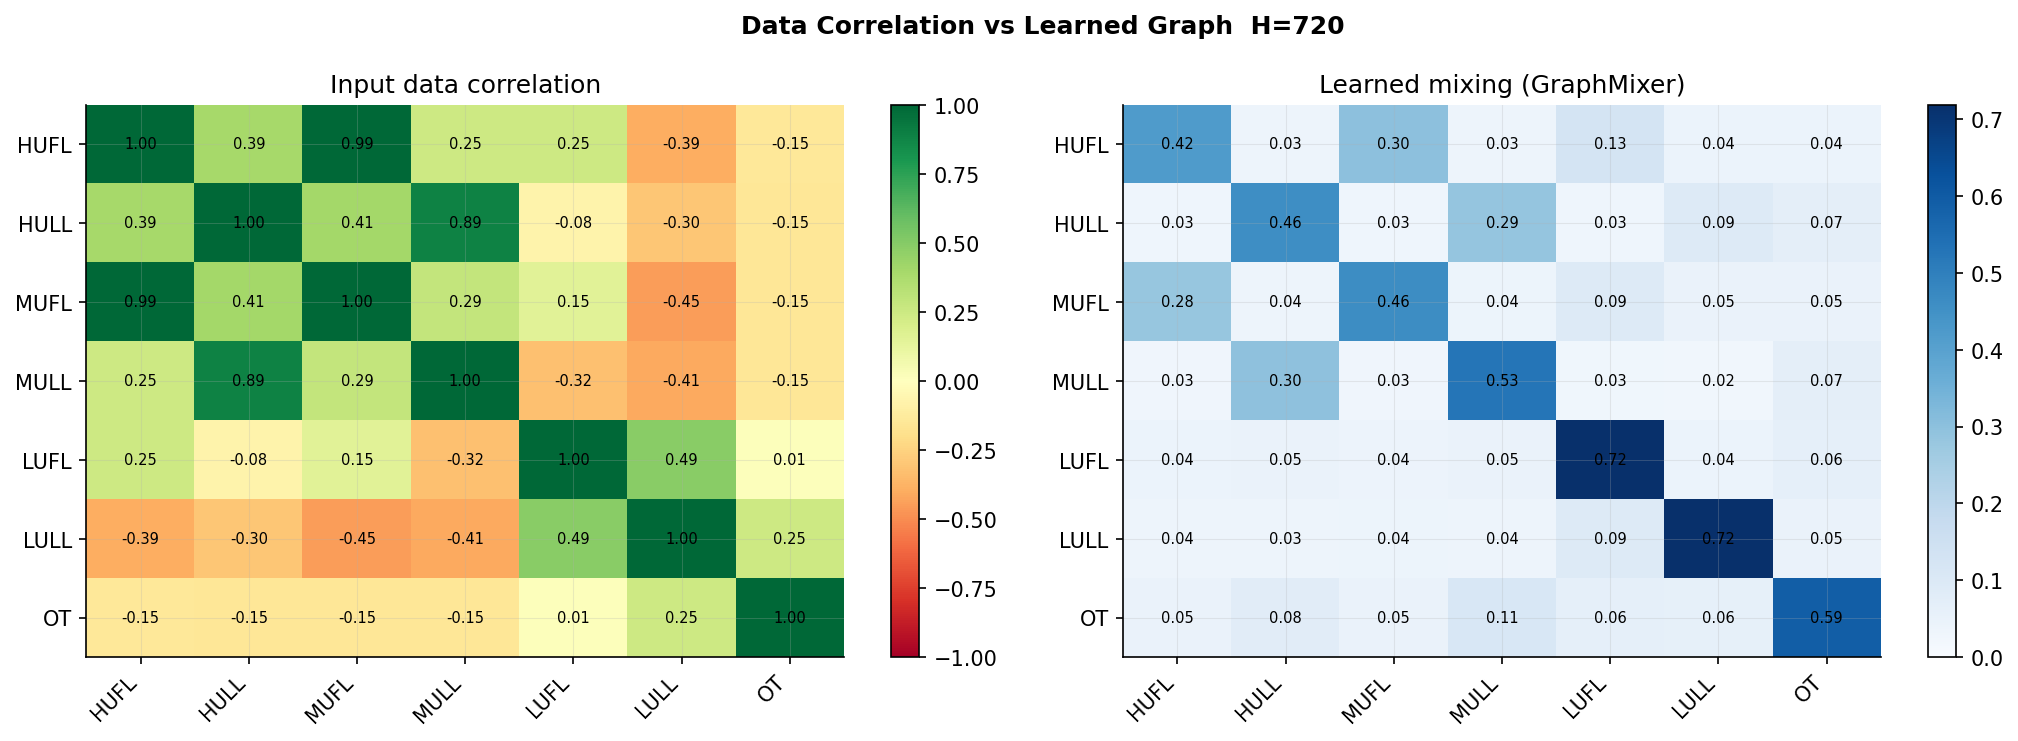
\includegraphics[width=\linewidth]{plots-old/variate_graph/correlation_vs_learned.png}
  \caption{Comparison of Pearson correlation matrix (empirical) against the learned variate interaction weights. High agreement indicates that P-WSA's shared-weight CI scheme implicitly encodes variate correlations through the training loss, even without explicit cross-variate attention.}
  \label{fig:corr-vs-learned}
\end{figure}

% ═════════════════════════════════════════════════════════════════════════════
\section{Model Complexity}
\label{sec:complexity}

With $d = 64$, $N_L = 3$, $P = 16$, $S = 8$, and $L = 336$, the number of trainable parameters is approximately 120--180K depending on the number of patches $N_p$. This is two to three orders of magnitude fewer parameters than large transformer models (e.g., iTransformer at $\approx$10M parameters), while remaining competitive on the ETTm1 benchmark. The inference complexity is $O(N_p \cdot d)$ per variate, scaling linearly with sequence length.

% ═════════════════════════════════════════════════════════════════════════════
\section{Design Rationale and Lessons Learned}
\label{sec:lessons}

Several design choices in v8.0 deviate from common practice and are worth explicating:

\begin{itemize}
  \item \textbf{No trend dropout.} Early versions applied dropout to the trend projection to prevent over-reliance on the moving average. This was observed to introduce baseline collapse in cases where the trend dominated the signal. Removing dropout from the trend path yielded consistent MSE improvements.
  \item \textbf{Low wavelet threshold initialisation.} An initialisation of $0.05$ (versus a common choice of $0.1$) was found to preserve more high-frequency detail in early epochs, allowing the network to learn which frequencies are informative rather than being pre-suppressed.
  \item \textbf{Zero input jitter.} Input noise augmentation can improve generalisation but introduces a calibration gap on deterministic test metrics. Since the primary evaluation criterion is MSE, jitter was disabled to provide a clean baseline. It can be re-enabled via the \texttt{--jitter} flag for robustness experiments.
  \item \textbf{Spectral + MSE combined loss.} Pure MSE training tends to produce over-smoothed predictions because the loss is minimised by predicting the conditional mean. The spectral penalty adds a direct supervision signal on the frequency content of predictions, counteracting this smoothing effect.
\end{itemize}

% ═════════════════════════════════════════════════════════════════════════════
\section{Conclusion}
\label{sec:conc}

P-WSA v8.0 shows that classical signal-processing priors can pair effectively with modern deep learning for multivariate time-series forecasting. Moving-average decomposition, instance normalisation, and wavelet multi-resolution analysis together deliver competitive results without expensive cross-channel attention. The ablation study shows that every proposed module helps, with the DWT orthogonality loss emerging as the most critical component. Future work will study cross-variate interaction layers, adaptive look-back window selection, and pre-training on large-scale time-series corpora.

% ═════════════════════════════════════════════════════════════════════════════
\section*{References}
\addcontentsline{toc}{section}{References}

\begin{enumerate}[label={[\arabic*]}]
  \item Kim, T., Kim, J., Tae, Y., Park, C., Choi, J.-H., \& Choo, J. (2022). \textit{Reversible Instance Normalization for Accurate Time-Series Forecasting against Distribution Shift}. ICLR 2022.
  \item Nie, Y., Nguyen, N.H., Sinthong, P., \& Kalagnanam, J. (2023). \textit{A Time Series is Worth 64 Words: Long-term Forecasting with Transformers}. ICLR 2023. (\textit{PatchTST})
  \item Tolstikhin, I., Houlsby, N., Kolesnikov, A., et al.\ (2021). \textit{MLP-Mixer: An all-MLP Architecture for Vision}. NeurIPS 2021.
  \item Liu, Y., Hu, T., Zhang, H., et al.\ (2023). \textit{iTransformer: Inverted Transformers Are Effective for Time Series Forecasting}. arXiv:2310.06625.
  \item Zhou, T., Ma, Z., Wen, Q., et al.\ (2022). \textit{FEDformer: Frequency Enhanced Decomposed Transformer for Long-term Series Forecasting}. ICML 2022.
  \item Zeng, A., Chen, M., Zhang, L., \& Xu, Q. (2023). \textit{Are Transformers Effective for Time Series Forecasting?} AAAI 2023. (\textit{DLinear})
\end{enumerate}

\end{document}